\documentclass[11pt]{article}
\usepackage[margin=1in]{geometry}
\usepackage[T1]{fontenc}
\usepackage[utf8]{inputenc}
\usepackage{lmodern}
\DeclareUnicodeCharacter{2295}{\ensuremath{\oplus}}
\DeclareUnicodeCharacter{00D7}{\ensuremath{\times}}
\DeclareUnicodeCharacter{00F7}{\ensuremath{\div}}
\DeclareUnicodeCharacter{2192}{\ensuremath{\to}}
\DeclareUnicodeCharacter{2264}{\ensuremath{\le}}
\usepackage{amsmath,amssymb}
\usepackage{booktabs}
\usepackage{graphicx}
\usepackage{xcolor}
\usepackage[numbers,sort&compress]{natbib}
\usepackage[colorlinks=true,linkcolor=blue!50!black,citecolor=blue!50!black,urlcolor=blue!50!black]{hyperref}
\usepackage{url}
\usepackage{enumitem}
\setlist{nosep,leftmargin=*}

% Small coloured change next to a score, as in Code2Video's tables. The colour says better or worse, not up or
% down: make_tables.delta() picks it from the column's direction (a drop on a lower-is-better column is \better),
% and columns with no better direction (sections rewritten, revisions used) get \neutral.
\definecolor{betterc}{HTML}{1F5FAD}\definecolor{worsec}{HTML}{C2491D}\definecolor{neutralc}{gray}{0.45}
\newcommand{\better}[1]{\,{\scriptsize\textcolor{betterc}{#1}}}
\newcommand{\worse}[1]{\,{\scriptsize\textcolor{worsec}{#1}}}
\newcommand{\neutral}[1]{\,{\scriptsize\textcolor{neutralc}{#1}}}
\newcommand{\hd}[1]{\begin{tabular}[b]{@{}c@{}}#1\end{tabular}}% a two-line table header

% A method figure generated from a prompt in figures/IMAGE_PROMPTS.md (Part A); a box names the prompt until the
% image file exists. Full text width in every document.
\newcommand{\paperfig}[4]{%
  \begin{figure*}[t]\centering
  \IfFileExists{figures/#1}{\includegraphics[width=\textwidth]{figures/#1}}{%
    \fbox{\parbox{0.92\textwidth}{\centering\small\vspace{22pt}\textit{Figure to generate: prompt #2 in}
    \texttt{paper/figures/IMAGE\_PROMPTS.md}, saved as \texttt{\detokenize{paper/figures/#1}}\vspace{22pt}}}}
  \caption{#3}\label{fig:#4}
  \end{figure*}}

% Every number below comes from paper/make_tables.py; a result that does not exist yet prints as [pending].
\newcommand{\pend}{\textcolor{red!70!black}{\textbf{[pending]}}}
\newcommand{\todo}[1]{\textcolor{red!70!black}{\textbf{[#1]}}}
\IfFileExists{tables/numbers.tex}{% generated by paper/make_tables.py; a missing macro means its result is pending
\newcommand{\AdmClean}{5}
\newcommand{\AdmComplete}{10}
\newcommand{\AdmIncompleteBefore}{7}
\newcommand{\AdmRegenerated}{23}
\newcommand{\AdmTotal}{12}
\newcommand{\AllRuns}{282}
\newcommand{\AnsweredRight}{103}
\newcommand{\AnsweredRightShare}{100}
\newcommand{\AnsweredWithVideo}{103}
\newcommand{\AnsweredWrong}{0}
\newcommand{\ClaudeCost}{2.35}
\newcommand{\ClaudeCrowded}{7}
\newcommand{\ClaudeFaults}{96}
\newcommand{\ClaudeLeftover}{10}
\newcommand{\ClaudeOffScreen}{11}
\newcommand{\ClaudeOther}{22}
\newcommand{\ClaudeOverlap}{42}
\newcommand{\ClaudeSections}{40}
\newcommand{\ClaudeUnreadable}{4}
\newcommand{\FailedAttempts}{241}
\newcommand{\FirstTryFail}{42}
\newcommand{\LSAutoAttach}{13}
\newcommand{\LSAutoConflicts}{29}
\newcommand{\LSAutoFrames}{67.5}
\newcommand{\LSAutoMNine}{42.4}
\newcommand{\LSAutoMSeven}{18.5}
\newcommand{\LSAutoMvqs}{84.2}
\newcommand{\LSClaudeAttach}{4}
\newcommand{\LSClaudeConflicts}{4}
\newcommand{\LSClaudeFrames}{69.8}
\newcommand{\LSClaudeMNine}{47.6}
\newcommand{\LSClaudeMSeven}{19.1}
\newcommand{\LSClaudeMvqs}{85.6}
\newcommand{\LSDiff}{+5.1}
\newcommand{\LSDiffWithoutTop}{$-$1.3}
\newcommand{\LSGate}{not passed}
\newcommand{\LSLeftOut}{0}
\newcommand{\LSLosses}{5}
\newcommand{\LSN}{10}
\newcommand{\LSNeed}{7}
\newcommand{\LSOursAttach}{13}
\newcommand{\LSOursConflicts}{31}
\newcommand{\LSOursFrames}{67.5}
\newcommand{\LSOursMNine}{42.4}
\newcommand{\LSOursMSeven}{17.6}
\newcommand{\LSOursMvqs}{84.2}
\newcommand{\LSTopDiff}{+62.7}
\newcommand{\LSTopTopic}{Sorrel counts of lattice rectangles}
\newcommand{\LSWins}{5}
\newcommand{\LadMMMCAbstained}{85}
\newcommand{\LadMMMCAgreeEight}{--}
\newcommand{\LadMMMCAgreeNine}{--}
\newcommand{\LadMMMCAgreeOne}{0.96}
\newcommand{\LadMMMCAgreeRawNine}{0.77}
\newcommand{\LadMMMCAgreeRawSeven}{0.65}
\newcommand{\LadMMMCAgreeSeven}{--}
\newcommand{\LadMMMCAgreeThree}{--}
\newcommand{\LadMMMCAgreeTwo}{1.00}
\newcommand{\LadMMMCBlindAllRight}{12}
\newcommand{\LadMMMCDefinedEight}{0/48}
\newcommand{\LadMMMCDefinedNVG}{0/48}
\newcommand{\LadMMMCDefinedNine}{0/48}
\newcommand{\LadMMMCDefinedOne}{47/48}
\newcommand{\LadMMMCDefinedRawNine}{48/48}
\newcommand{\LadMMMCDefinedRawSeven}{48/48}
\newcommand{\LadMMMCDefinedSeven}{0/48}
\newcommand{\LadMMMCDefinedThree}{0/48}
\newcommand{\LadMMMCDefinedTwo}{48/48}
\newcommand{\LadMMMCLAEight}{--}
\newcommand{\LadMMMCLANine}{--}
\newcommand{\LadMMMCLAOne}{+0.6}
\newcommand{\LadMMMCLARawNine}{+0.1}
\newcommand{\LadMMMCLARawSeven}{+0.3}
\newcommand{\LadMMMCLASeven}{--}
\newcommand{\LadMMMCLAThree}{--}
\newcommand{\LadMMMCLATwo}{0.0}
\newcommand{\LadMMMCLBEight}{--}
\newcommand{\LadMMMCLBNine}{--}
\newcommand{\LadMMMCLBOne}{+7.2}
\newcommand{\LadMMMCLBRawNine}{+0.1}
\newcommand{\LadMMMCLBRawSeven}{+1.4}
\newcommand{\LadMMMCLBSeven}{--}
\newcommand{\LadMMMCLBThree}{--}
\newcommand{\LadMMMCLBTwo}{0.0}
\newcommand{\LadMMMCLGEight}{--}
\newcommand{\LadMMMCLGNine}{--}
\newcommand{\LadMMMCLGOne}{+2.8}
\newcommand{\LadMMMCLGRawNine}{0.0}
\newcommand{\LadMMMCLGRawSeven}{$-$0.1}
\newcommand{\LadMMMCLGSeven}{--}
\newcommand{\LadMMMCLGThree}{--}
\newcommand{\LadMMMCLGTwo}{0.0}
\newcommand{\LadMMMCSBlind}{100.0}
\newcommand{\LadMMMCSFrames}{98.3}
\newcommand{\LadMMMCSStatic}{98.8}
\newcommand{\LadMMMCSVisual}{99.4}
\newcommand{\LadMMMCSepEight}{--}
\newcommand{\LadMMMCSepNine}{--}
\newcommand{\LadMMMCSepOne}{+10.6}
\newcommand{\LadMMMCSepRawNine}{+13.0}
\newcommand{\LadMMMCSepRawSeven}{+4.1}
\newcommand{\LadMMMCSepSeven}{--}
\newcommand{\LadMMMCSepThree}{--}
\newcommand{\LadMMMCSepTwo}{+16.7}
\newcommand{\LadMMMCTiesEight}{--}
\newcommand{\LadMMMCTiesNine}{--}
\newcommand{\LadMMMCTiesOne}{7}
\newcommand{\LadMMMCTiesRawNine}{0}
\newcommand{\LadMMMCTiesRawSeven}{1}
\newcommand{\LadMMMCTiesSeven}{--}
\newcommand{\LadMMMCTiesThree}{--}
\newcommand{\LadMMMCTiesTwo}{12}
\newcommand{\LadMMMCTopics}{12}
\newcommand{\LadMMMCVideos}{48}
\newcommand{\LadNovelAbstained}{42}
\newcommand{\LadNovelAgreeEight}{--}
\newcommand{\LadNovelAgreeNine}{--}
\newcommand{\LadNovelAgreeOne}{0.67}
\newcommand{\LadNovelAgreeRawNine}{0.30}
\newcommand{\LadNovelAgreeRawSeven}{-0.31}
\newcommand{\LadNovelAgreeSeven}{--}
\newcommand{\LadNovelAgreeThree}{0.43}
\newcommand{\LadNovelAgreeTwo}{0.21}
\newcommand{\LadNovelBlindAllRight}{0}
\newcommand{\LadNovelDefinedEight}{10/10}
\newcommand{\LadNovelDefinedNVG}{10/10}
\newcommand{\LadNovelDefinedNine}{10/10}
\newcommand{\LadNovelDefinedOne}{10/10}
\newcommand{\LadNovelDefinedRawNine}{10/10}
\newcommand{\LadNovelDefinedRawSeven}{10/10}
\newcommand{\LadNovelDefinedSeven}{10/10}
\newcommand{\LadNovelDefinedThree}{10/10}
\newcommand{\LadNovelDefinedTwo}{10/10}
\newcommand{\LadNovelLAEight}{--}
\newcommand{\LadNovelLANine}{--}
\newcommand{\LadNovelLAOne}{--}
\newcommand{\LadNovelLARawNine}{--}
\newcommand{\LadNovelLARawSeven}{--}
\newcommand{\LadNovelLASeven}{--}
\newcommand{\LadNovelLAThree}{--}
\newcommand{\LadNovelLATwo}{--}
\newcommand{\LadNovelLBEight}{--}
\newcommand{\LadNovelLBNine}{--}
\newcommand{\LadNovelLBOne}{--}
\newcommand{\LadNovelLBRawNine}{--}
\newcommand{\LadNovelLBRawSeven}{--}
\newcommand{\LadNovelLBSeven}{--}
\newcommand{\LadNovelLBThree}{--}
\newcommand{\LadNovelLBTwo}{--}
\newcommand{\LadNovelLGEight}{--}
\newcommand{\LadNovelLGNine}{--}
\newcommand{\LadNovelLGOne}{--}
\newcommand{\LadNovelLGRawNine}{--}
\newcommand{\LadNovelLGRawSeven}{--}
\newcommand{\LadNovelLGSeven}{--}
\newcommand{\LadNovelLGThree}{--}
\newcommand{\LadNovelLGTwo}{--}
\newcommand{\LadNovelSBlind}{41.0}
\newcommand{\LadNovelSFrames}{67.5}
\newcommand{\LadNovelSStatic}{47.1}
\newcommand{\LadNovelSVisual}{50.2}
\newcommand{\LadNovelSepEight}{+26.5}
\newcommand{\LadNovelSepNine}{+64.4}
\newcommand{\LadNovelSepOne}{+48.3}
\newcommand{\LadNovelSepRawNine}{+36.2}
\newcommand{\LadNovelSepRawSeven}{+12.1}
\newcommand{\LadNovelSepSeven}{+26.5}
\newcommand{\LadNovelSepThree}{+74.5}
\newcommand{\LadNovelSepTwo}{+42.5}
\newcommand{\LadNovelTiesEight}{--}
\newcommand{\LadNovelTiesNine}{--}
\newcommand{\LadNovelTiesOne}{--}
\newcommand{\LadNovelTiesRawNine}{--}
\newcommand{\LadNovelTiesRawSeven}{--}
\newcommand{\LadNovelTiesSeven}{--}
\newcommand{\LadNovelTiesThree}{--}
\newcommand{\LadNovelTiesTwo}{--}
\newcommand{\LadNovelTopics}{10}
\newcommand{\LadNovelVideos}{10}
\newcommand{\LadSmallAbstained}{--}
\newcommand{\LadSmallAgreeEight}{--}
\newcommand{\LadSmallAgreeNine}{--}
\newcommand{\LadSmallAgreeOne}{--}
\newcommand{\LadSmallAgreeRawNine}{0.70}
\newcommand{\LadSmallAgreeRawSeven}{--}
\newcommand{\LadSmallAgreeSeven}{--}
\newcommand{\LadSmallAgreeThree}{0.72}
\newcommand{\LadSmallAgreeTwo}{0.65}
\newcommand{\LadSmallBlindAllRight}{6}
\newcommand{\LadSmallDefinedEight}{0/48}
\newcommand{\LadSmallDefinedNVG}{24/48}
\newcommand{\LadSmallDefinedNine}{36/48}
\newcommand{\LadSmallDefinedOne}{0/48}
\newcommand{\LadSmallDefinedRawNine}{48/48}
\newcommand{\LadSmallDefinedRawSeven}{0/48}
\newcommand{\LadSmallDefinedSeven}{0/48}
\newcommand{\LadSmallDefinedThree}{24/48}
\newcommand{\LadSmallDefinedTwo}{48/48}
\newcommand{\LadSmallLAEight}{--}
\newcommand{\LadSmallLANine}{+5.9}
\newcommand{\LadSmallLAOne}{--}
\newcommand{\LadSmallLARawNine}{+1.2}
\newcommand{\LadSmallLARawSeven}{--}
\newcommand{\LadSmallLASeven}{--}
\newcommand{\LadSmallLAThree}{+16.7}
\newcommand{\LadSmallLATwo}{+3.3}
\newcommand{\LadSmallLBEight}{--}
\newcommand{\LadSmallLBNine}{$-$23.7}
\newcommand{\LadSmallLBOne}{--}
\newcommand{\LadSmallLBRawNine}{$-$2.9}
\newcommand{\LadSmallLBRawSeven}{--}
\newcommand{\LadSmallLBSeven}{--}
\newcommand{\LadSmallLBThree}{+25.0}
\newcommand{\LadSmallLBTwo}{$-$3.3}
\newcommand{\LadSmallLGEight}{--}
\newcommand{\LadSmallLGNine}{$-$0.6}
\newcommand{\LadSmallLGOne}{--}
\newcommand{\LadSmallLGRawNine}{+0.2}
\newcommand{\LadSmallLGRawSeven}{--}
\newcommand{\LadSmallLGSeven}{--}
\newcommand{\LadSmallLGThree}{+8.3}
\newcommand{\LadSmallLGTwo}{+1.7}
\newcommand{\LadSmallSBlind}{81.7}
\newcommand{\LadSmallSFrames}{77.0}
\newcommand{\LadSmallSepEight}{--}
\newcommand{\LadSmallSepNine}{+37.9}
\newcommand{\LadSmallSepOne}{--}
\newcommand{\LadSmallSepRawNine}{+6.4}
\newcommand{\LadSmallSepRawSeven}{--}
\newcommand{\LadSmallSepSeven}{--}
\newcommand{\LadSmallSepThree}{+16.7}
\newcommand{\LadSmallSepTwo}{+10.0}
\newcommand{\LadSmallTiesEight}{--}
\newcommand{\LadSmallTiesNine}{1}
\newcommand{\LadSmallTiesOne}{--}
\newcommand{\LadSmallTiesRawNine}{1}
\newcommand{\LadSmallTiesRawSeven}{--}
\newcommand{\LadSmallTiesSeven}{--}
\newcommand{\LadSmallTiesThree}{4}
\newcommand{\LadSmallTiesTwo}{9}
\newcommand{\LadSmallTopics}{12}
\newcommand{\LadSmallVideos}{48}
\newcommand{\NMDense}{+14.1}
\newcommand{\NMDenseMDE}{28.0}
\newcommand{\NMDenseN}{10}
\newcommand{\NMDensePos}{9}
\newcommand{\NMFloorAll}{1.9}
\newcommand{\NMFloorOne}{7.2}
\newcommand{\NMFramesDense}{+28.4}
\newcommand{\NMFramesDenseMDE}{37.7}
\newcommand{\NMFramesDenseN}{10}
\newcommand{\NMFramesDensePos}{8}
\newcommand{\NMGain}{+42.4}
\newcommand{\NMGainMDE}{39.4}
\newcommand{\NMGainN}{10}
\newcommand{\NMGainPos}{9}
\newcommand{\NMLayout}{+5.1}
\newcommand{\NMLayoutMDE}{24.2}
\newcommand{\NMLayoutN}{10}
\newcommand{\NMLayoutPos}{5}
\newcommand{\NMRepeatMoved}{33}
\newcommand{\NMRepeatN}{232}
\newcommand{\NMRuleFPR}{8.2}
\newcommand{\NMSmall}{$-$23.7}
\newcommand{\NMSmallMDE}{160.2}
\newcommand{\NMSmallN}{9}
\newcommand{\NMSmallPos}{5}
\newcommand{\NMSpec}{+64.4}
\newcommand{\NMSpecMDE}{42.7}
\newcommand{\NMSpecN}{10}
\newcommand{\NMSpecPos}{10}
\newcommand{\NovelItems}{96}
\newcommand{\NovelUnknown}{58}
\newcommand{\NullNoVideo}{100}
\newcommand{\NullWithVideo}{85}
\newcommand{\NullWithVideoN}{602}
\newcommand{\OrderRuns}{146}
\newcommand{\OrderShare}{52}
\newcommand{\PilotDev}{127}
\newcommand{\PilotDevGain}{+12.2}
\newcommand{\PilotFlagged}{3.3}
\newcommand{\PilotGaps}{124}
\newcommand{\PilotLayoutAll}{72.6}
\newcommand{\PilotLayoutBase}{78.5}
\newcommand{\PilotNotKept}{9}
\newcommand{\PilotRevisions}{36}
\newcommand{\PilotSections}{4}
\newcommand{\PilotTies}{7}
\newcommand{\PreflightFP}{1}
\newcommand{\PreflightN}{156}
\newcommand{\ShiftNotes}{25}
\newcommand{\ShiftsIn}{41}
\newcommand{\ShiftsRemoved}{38}
\newcommand{\SyntaxAfterPatch}{38}
\newcommand{\mmmcpriorGemmaAcc}{99.0}
\newcommand{\mmmcpriorGemmaAllRight}{108}
\newcommand{\mmmcpriorGemmaP}{99.0}
\newcommand{\mmmcpriorGemmaTopics}{117}
\newcommand{\mmmcpriorQwenAcc}{97.4}
\newcommand{\mmmcpriorQwenAllRight}{99}
\newcommand{\mmmcpriorQwenP}{95.6}
\newcommand{\mmmcpriorQwenSmallAcc}{91.9}
\newcommand{\mmmcpriorQwenSmallAllRight}{67}
\newcommand{\mmmcpriorQwenSmallP}{86.6}
\newcommand{\mmmcpriorQwenSmallTopics}{117}
\newcommand{\mmmcpriorQwenTopics}{117}
\newcommand{\novelcardGemmaAcc}{84.9}
\newcommand{\novelcardGemmaAllRight}{1}
\newcommand{\novelcardGemmaP}{83.7}
\newcommand{\novelcardGemmaTopics}{12}
\newcommand{\novelpriorGemmaAcc}{41.1}
\newcommand{\novelpriorGemmaAllRight}{0}
\newcommand{\novelpriorGemmaP}{41.4}
\newcommand{\novelpriorGemmaTopics}{12}
}{}
\providecommand{\AllRuns}{\pend}\providecommand{\OrderRuns}{\pend}\providecommand{\OrderShare}{\pend}
\providecommand{\NullWithVideo}{\pend}\providecommand{\NullNoVideo}{\pend}\providecommand{\PilotTies}{\pend}
\providecommand{\FailedAttempts}{\pend}\providecommand{\FirstTryFail}{\pend}
\providecommand{\PreflightFP}{\pend}\providecommand{\PilotNotKept}{\pend}\providecommand{\PilotRevisions}{\pend}\providecommand{\PreflightN}{\pend}\providecommand{\SyntaxAfterPatch}{\pend}\providecommand{\PilotGaps}{\pend}\providecommand{\PilotDev}{\pend}\providecommand{\PilotFlagged}{\pend}\providecommand{\PilotSections}{\pend}\providecommand{\PilotDevGain}{\pend}
\providecommand{\mmmcpriorGemmaAcc}{\pend}\providecommand{\mmmcpriorGemmaP}{\pend}
\providecommand{\mmmcpriorGemmaAllRight}{\pend}\providecommand{\mmmcpriorGemmaTopics}{\pend}
\providecommand{\mmmcpriorQwenAcc}{\pend}\providecommand{\mmmcpriorQwenSmallAcc}{\pend}\providecommand{\mmmcpriorQwenP}{\pend}
\providecommand{\novelpriorGemmaAcc}{\pend}\providecommand{\novelpriorGemmaP}{\pend}
\providecommand{\novelcardGemmaAcc}{\pend}\providecommand{\novelcardGemmaP}{\pend}
\providecommand{\LadMMMCBlindAllRight}{\pend}\providecommand{\LadMMMCTopics}{\pend}\providecommand{\LadMMMCAbstained}{\pend}
\providecommand{\LadMMMCVideos}{\pend}\providecommand{\LadMMMCSepOne}{\pend}\providecommand{\LadMMMCSepTwo}{\pend}\providecommand{\LadMMMCLBOne}{\pend}\providecommand{\LadMMMCLBTwo}{\pend}\providecommand{\LadMMMCTiesOne}{\pend}\providecommand{\LadMMMCTiesTwo}{\pend}\providecommand{\LadMMMCDefinedNVG}{\pend}
\providecommand{\LadSmallSBlind}{\pend}\providecommand{\LadSmallDefinedNine}{\pend}\providecommand{\LadSmallSepNine}{\pend}\providecommand{\LadSmallSepRawNine}{\pend}\providecommand{\LadSmallLBNine}{\pend}\providecommand{\LadSmallLBRawNine}{\pend}\providecommand{\LadSmallLGNine}{\pend}\providecommand{\LadMMMCSBlind}{\pend}\providecommand{\LadMMMCSVisual}{\pend}\providecommand{\LadMMMCSepRawNine}{\pend}
\providecommand{\LadNovelSBlind}{\pend}\providecommand{\LadNovelDefinedNine}{\pend}\providecommand{\LadNovelSepNine}{\pend}\providecommand{\LadNovelDefinedSeven}{\pend}\providecommand{\LadNovelSepSeven}{\pend}\providecommand{\LadNovelSFrames}{\pend}\providecommand{\LadNovelSVisual}{\pend}\providecommand{\AdmIncompleteBefore}{\pend}\providecommand{\AdmTotal}{\pend}\providecommand{\AdmComplete}{\pend}\providecommand{\AdmClean}{\pend}\providecommand{\ClaudeFaults}{\pend}\providecommand{\ClaudeSections}{\pend}\providecommand{\ClaudeCost}{\pend}\providecommand{\ClaudeOverlap}{\pend}\providecommand{\ClaudeOther}{\pend}\providecommand{\ClaudeOffScreen}{\pend}\providecommand{\ClaudeLeftover}{\pend}\providecommand{\ClaudeCrowded}{\pend}\providecommand{\ClaudeUnreadable}{\pend}\providecommand{\ShiftsIn}{\pend}\providecommand{\ShiftsRemoved}{\pend}\providecommand{\ShiftNotes}{\pend}\providecommand{\LSDiff}{\pend}\providecommand{\LSWins}{\pend}\providecommand{\LSN}{\pend}\providecommand{\LSGate}{\pend}
\providecommand{\LadNovelBlindAllRight}{\pend}\providecommand{\LadNovelTopics}{\pend}\providecommand{\LadNovelAbstained}{\pend}

\newcommand{\Sblind}{S_{\text{none}}}
\newcommand{\Sstatic}{S_{\text{static}}}
\newcommand{\Svisual}{S_{\text{visual}}}
\newcommand{\Beff}{B_{\text{eff}}}
% noise model (bench/noise_model.py), filled by make_tables.py
\providecommand{\LSOursConflicts}{\pend}\providecommand{\LSClaudeConflicts}{\pend}\providecommand{\LSOursAttach}{\pend}\providecommand{\LSClaudeAttach}{\pend}\providecommand{\LSOursMvqs}{\pend}\providecommand{\LSClaudeMvqs}{\pend}\providecommand{\NMRepeatMoved}{\pend}\providecommand{\NMRepeatN}{\pend}\providecommand{\NMFloorOne}{\pend}\providecommand{\NMFloorAll}{\pend}\providecommand{\NMGain}{\pend}\providecommand{\NMGainPos}{\pend}\providecommand{\NMGainN}{\pend}\providecommand{\NMSpec}{\pend}\providecommand{\NMSpecPos}{\pend}\providecommand{\NMSpecN}{\pend}\providecommand{\NMFramesDense}{\pend}\providecommand{\NMFramesDensePos}{\pend}\providecommand{\NMFramesDenseN}{\pend}\providecommand{\NMLayoutMDE}{\pend}\providecommand{\NMRuleFPR}{\pend}\providecommand{\NMSmallMDE}{\pend}

\usepackage[section]{placeins}
\usepackage{tikz}
\usetikzlibrary{arrows.meta,positioning,shapes.geometric,fit,calc}
\usepackage[most]{tcolorbox}
\newtcolorbox{inshort}{colback=blue!4,colframe=blue!40!black,boxrule=0.6pt,arc=2pt,left=6pt,right=6pt,top=4pt,bottom=4pt,
  fonttitle=\bfseries\small,title=In short}
\newtcolorbox{example}[1][]{colback=gray!5,colframe=gray!50,boxrule=0.5pt,arc=2pt,left=6pt,right=6pt,top=4pt,bottom=4pt,
  fonttitle=\bfseries\small,title=Example#1}
\setlength{\parskip}{4pt}
% Conceptual diagrams for the long report (TikZ). Data figures come from make_figures.py; illustrations from the
% prompts in figures/IMAGE_PROMPTS.md (\imageslot shows the prompt id until the image file exists).

\tikzset{
  box/.style={draw, rounded corners=2pt, fill=blue!5, minimum height=0.75cm, align=center, font=\small},
  ours/.style={draw, rounded corners=2pt, fill=orange!14, minimum height=0.75cm, align=center, font=\small},
  bad/.style={draw, rounded corners=2pt, fill=red!8, minimum height=0.75cm, align=center, font=\small},
  note/.style={font=\footnotesize, align=center, text=black!70},
  >={Stealth}
}

% An illustration to be generated from a prompt; until the file exists, a box names the prompt.
\newcommand{\imageslot}[3]{%
  \begin{figure}[htbp]\centering
  \IfFileExists{figures/#1}{\includegraphics[width=0.62\linewidth]{figures/#1}}{%
    \fbox{\parbox{0.62\linewidth}{\centering\small\vspace{14pt}\textit{Illustration to generate: prompt #2 in}\\
    \texttt{paper/figures/IMAGE\_PROMPTS.md}, saved as \texttt{paper/figures/#1}\vspace{14pt}}}}
  \caption{#3}
  \end{figure}}

% A data figure from make_figures.py; a pending box until its data exists.
\newcommand{\datafig}[3][0.9]{%
  \begin{figure}[htbp]\centering
  \IfFileExists{figures/#2.pdf}{\includegraphics[width=#1\linewidth]{figures/#2.pdf}}{%
    \fbox{\parbox{0.8\linewidth}{\centering\small\textit{Pending: this figure is drawn when its run finishes.}}}}
  \caption{#3}\label{fig:#2}
  \end{figure}}

\newcommand{\DiagTeachQuiz}{%
\begin{figure}[htbp]\centering
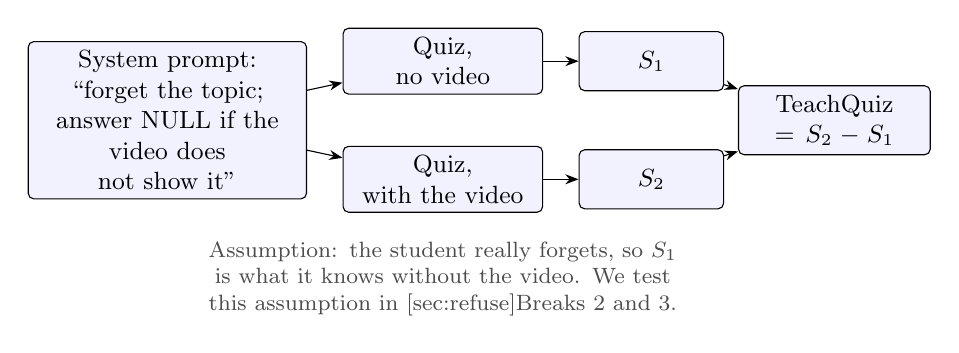
\begin{tikzpicture}[node distance=0.4cm and 0.45cm]
\node[box, text width=3.3cm] (p) {System prompt:\\``forget the topic;\\answer NULL if the\\video does not show it''};
\node[box, right=of p, text width=2.3cm, yshift=0.75cm] (a1) {Quiz,\\no video};
\node[box, right=of p, text width=2.3cm, yshift=-0.75cm] (a2) {Quiz,\\with the video};
\node[box, right=of a1, text width=1.6cm] (s1) {$S_1$};
\node[box, right=of a2, text width=1.6cm] (s2) {$S_2$};
\node[box, right=1.1cm of $(s1)!0.5!(s2)$, text width=2.2cm] (tq) {TeachQuiz\\$= S_2 - S_1$};
\draw[->] (p) -- (a1); \draw[->] (p) -- (a2); \draw[->] (a1) -- (s1); \draw[->] (a2) -- (s2);
\draw[->] (s1) -- (tq); \draw[->] (s2) -- (tq);
\node[note, below=0.25cm of a2, text width=9cm] {Assumption: the student really forgets, so $S_1$ is what it knows
without the video. We test this assumption in \hyperref[sec:refuse]{Breaks 2 and 3}.};
\end{tikzpicture}
\caption{How Code2Video's TeachQuiz measures teaching.}\label{fig:teachquiz}
\end{figure}}

\newcommand{\DiagDVGAIN}{%
\begin{figure}[htbp]\centering
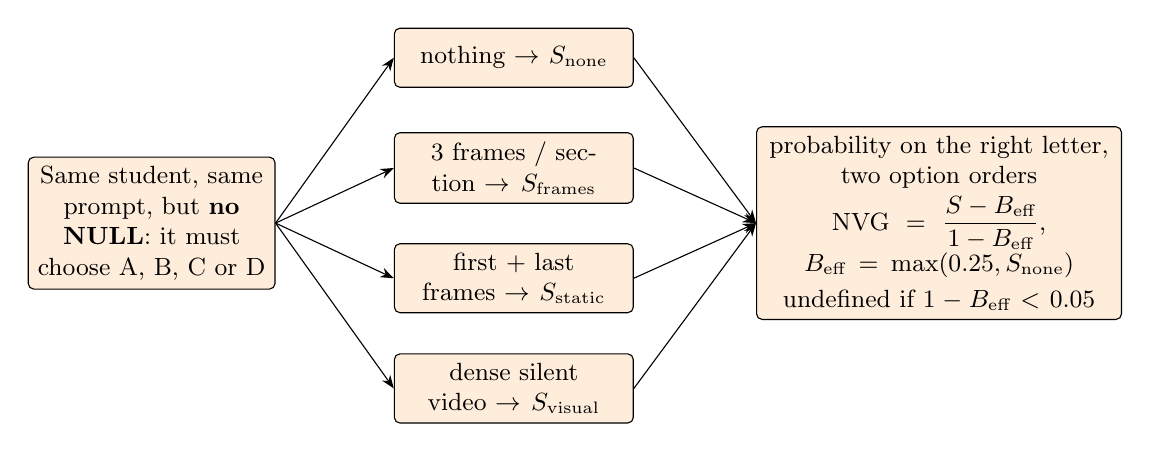
\begin{tikzpicture}[node distance=0.35cm and 0.45cm]
\node[ours, text width=2.9cm] (p) at (0,0) {Same student, same prompt, but \textbf{no NULL}: it must choose A, B, C or D};
\node[ours, text width=2.8cm] (b) at (4.6, 2.1) {nothing $\to S_{\text{none}}$};
\node[ours, text width=2.8cm] (f) at (4.6, 0.7) {3 frames / section $\to S_{\text{frames}}$};
\node[ours, text width=2.8cm] (s) at (4.6, -0.7) {first + last frames $\to S_{\text{static}}$};
\node[ours, text width=2.8cm] (v) at (4.6, -2.1) {dense silent video $\to S_{\text{visual}}$};
\node[ours, text width=4.4cm] (m) at (10.0, 0)
  {probability on the right letter,\\two option orders\\[2pt]
   $\mathrm{NVG} = \dfrac{S - B_{\text{eff}}}{1 - B_{\text{eff}}}$, $B_{\text{eff}} = \max(0.25, S_{\text{none}})$\\[2pt]
   undefined if $1 - B_{\text{eff}} < 0.05$};
\foreach \n in {b,f,s,v} {\draw[->] (p.east) -- (\n.west); \draw[->] (\n.east) -- (m.west);}
\end{tikzpicture}
\caption{How we measure: the prior is measured, not wished away, and the materials separate what the student
knew, what sharp frames show, what start/end states show, and what the animation shows.}\label{fig:dvgain}
\end{figure}}

\newcommand{\DiagIdBug}{%
\begin{figure}[htbp]\centering
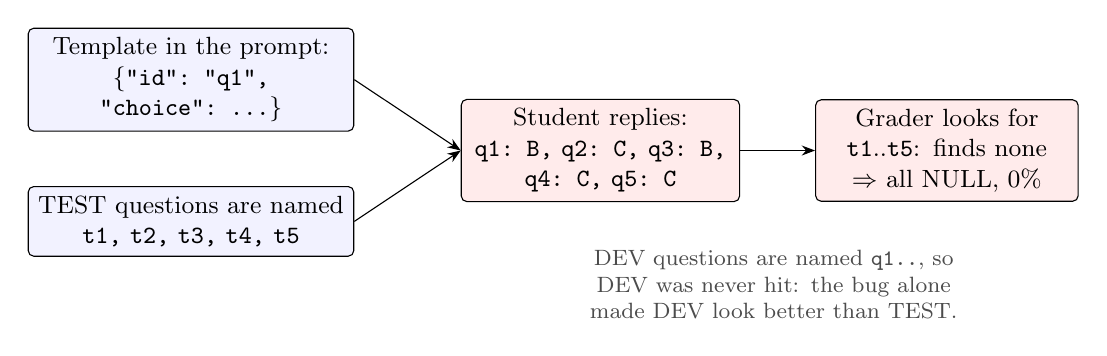
\begin{tikzpicture}[node distance=0.35cm and 0.55cm]
\node[box, text width=3.9cm] (tpl) at (0, 0.9) {Template in the prompt:\\\texttt{\{"id": "q1", "choice": ...\}}};
\node[box, text width=3.9cm] (qs) at (0, -0.9) {TEST questions are named\\\texttt{t1, t2, t3, t4, t5}};
\node[bad, text width=3.3cm] (rep) at (5.2, 0) {Student replies:\\\texttt{q1: B, q2: C, q3: B,}\\\texttt{q4: C, q5: C}};
\node[bad, text width=3.1cm] (gr) at (9.6, 0) {Grader looks for \texttt{t1}..\texttt{t5}: finds none $\Rightarrow$ all NULL, 0\%};
\draw[->] (tpl.east) -- (rep.west); \draw[->] (qs.east) -- (rep.west); \draw[->] (rep) -- (gr);
\node[note, text width=6cm] at (7.4, -1.7) {DEV questions are named \texttt{q1..}, so DEV was
never hit: the bug alone made DEV look better than TEST.};
\end{tikzpicture}
\caption{The grading bug (\hyperref[sec:idbug]{Break 1}). Fixed by matching answers in order when no id matches.}\label{fig:idbug}
\end{figure}}

\newcommand{\DiagDevTest}{%
\begin{figure}[htbp]\centering
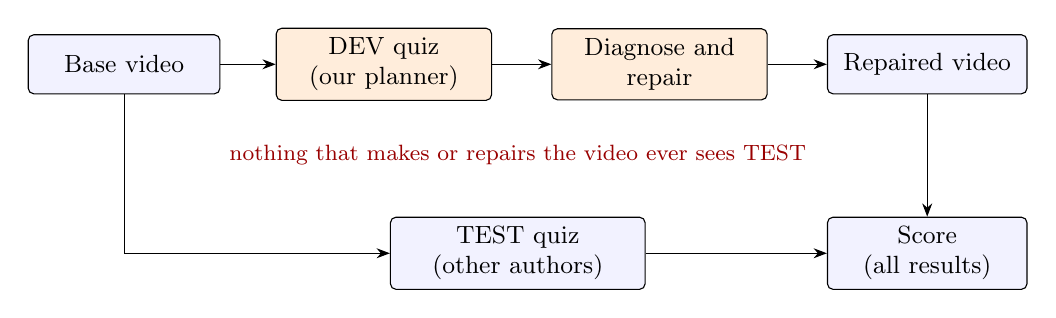
\begin{tikzpicture}
\node[box, text width=2.2cm] (v) at (0, 0) {Base video};
\node[ours, text width=2.5cm] (dev) at (3.3, 0) {DEV quiz\\(our planner)};
\node[ours, text width=2.5cm] (fix) at (6.8, 0) {Diagnose and\\repair};
\node[box, text width=2.3cm] (v2) at (10.2, 0) {Repaired video};
\node[box, text width=3.0cm] (test) at (5.0, -2.4) {TEST quiz\\(other authors)};
\node[box, text width=2.3cm] (score) at (10.2, -2.4) {Score\\(all results)};
\draw[->] (v) -- (dev); \draw[->] (dev) -- (fix); \draw[->] (fix) -- (v2); \draw[->] (v2) -- (score);
\draw[->] (v.south) |- (test.west); \draw[->] (test) -- (score);
\draw[red!60!black, thick, dashed] (1.6, -1.15) -- (8.6, -1.15);
\node[font=\footnotesize, text=red!60!black, fill=white] at (5.0, -1.15) {nothing that makes or repairs the video ever sees TEST};
\end{tikzpicture}
\caption{Two quizzes that never mix. The repair may look at DEV; every result is measured on TEST.}\label{fig:devtest}
\end{figure}}

\newcommand{\DiagSBFL}{%
\begin{figure}[htbp]\centering
\small
\begin{tabular}{l|cccc|c}
\toprule
Practice question & s1 & s2 & s3 & s4 & Student \\
\midrule
q1 & \textbullet & & & & passed \\
q2 & & \textbullet & & & \textcolor{red!60!black}{failed} \\
q3 & & \textbullet & & & \textcolor{red!60!black}{failed} \\
q4 & & \textbullet & & & passed \\
q5 & & & \textbullet & & \textcolor{red!60!black}{failed} \\
\midrule
failed / passed mapped & 0 / 1 & 2 / 1 & 1 / 0 & 0 / 0 & $F = 3$ \\
Ochiai $e_f/\sqrt{F(e_f+e_p)}$ & 0 & \textbf{0.67} & 0.58 & 0 & \\
\bottomrule
\end{tabular}
\caption{Spectrum-based localisation, an illustrative example. Each practice question is mapped to the section that
should teach it (a Q-matrix). A section is suspicious when the questions it should teach fail and the others pass;
here s2 is repaired first, then s3 if the budget allows two. The pilot's diagnosis instead flagged almost every
section, because it saw only failures.}\label{fig:sbfl}
\end{figure}}

\newcommand{\DiagLadder}{%
\begin{figure}[htbp]\centering
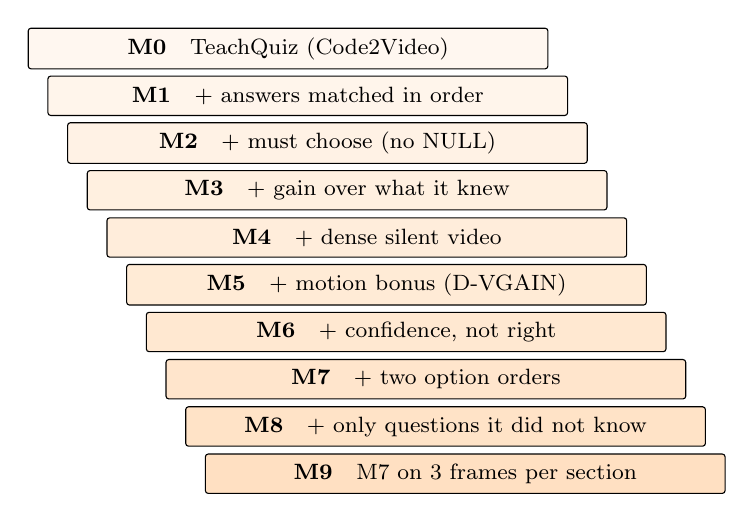
\begin{tikzpicture}[node distance=0.12cm, every node/.style={font=\footnotesize}]
\foreach \i/\t [count=\k] in {M0/TeachQuiz (Code2Video), M1/+ answers matched in order, M2/+ must choose (no NULL),
  M3/+ gain over what it knew, M4/+ dense silent video, M5/+ motion bonus (D-VGAIN), M6/+ confidence{,} not right/wrong,
  M7/+ two option orders, M8/+ only questions it did not know, M9/M7 on 3 frames per section} {
  \node[draw, rounded corners=1pt, fill=orange!\the\numexpr 4+\k*2\relax, minimum width=6.6cm, minimum height=0.5cm,
        anchor=west] at (\k*0.25, -\k*0.6) {\textbf{\i}\quad \t};
}
\end{tikzpicture}
\caption{The metric ladder. Each version of the measure changes one thing; every version is judged by the same four tests on the same
videos.}\label{fig:ladder}
\end{figure}}

% The study in four steps (every number is a macro from make_tables.py).
\newcommand{\DiagStudy}{%
\begin{figure}[htbp]\centering
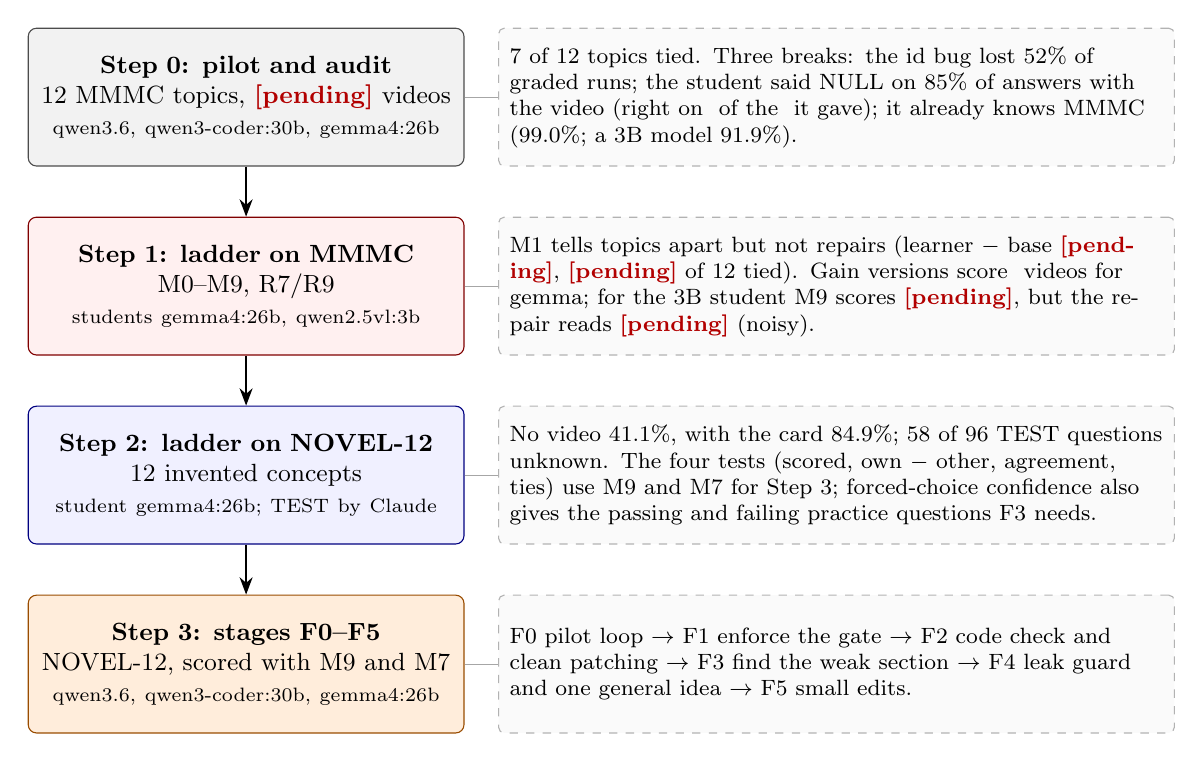
\begin{tikzpicture}[every node/.style={font=\small},
  stage/.style={draw, rounded corners=3pt, text width=5.3cm, minimum height=1.75cm, align=center},
  s0/.style={stage, fill=gray!10, draw=gray!60!black}, s1/.style={stage, fill=red!6, draw=red!50!black},
  s2/.style={stage, fill=blue!6, draw=blue!50!black}, s3/.style={stage, fill=orange!14, draw=orange!60!black},
  snote/.style={draw=gray!60, dashed, rounded corners=2pt, fill=gray!4, text width=8.3cm, align=left, inner sep=4pt,
    font=\footnotesize, minimum height=1.75cm},
  >={Stealth[length=2.2mm]}]
\node[s0] (p0) at (0, 0) {\textbf{Step 0: pilot and audit}\\12 MMMC topics, \LadMMMCVideos{} videos\\{\scriptsize qwen3.6, qwen3-coder:30b, gemma4:26b}};
\node[snote, anchor=west] (n0) at (3.2, 0) {\PilotTies{} of 12 topics tied. Three breaks: the id bug lost
  \OrderShare\% of graded runs; the student said NULL on \NullWithVideo\% of answers with the video (right on
  \AnsweredRight{} of the \AnsweredWithVideo{} it gave); it already knows MMMC (\mmmcpriorGemmaAcc\%; a 3B model
  \mmmcpriorQwenSmallAcc\%).};
\node[s1] (p1) at (0, -2.4) {\textbf{Step 1: ladder on MMMC}\\M0--M9, R7/R9\\{\scriptsize students gemma4:26b, qwen2.5vl:3b}};
\node[snote, anchor=west] (n1) at (3.2, -2.4) {M1 tells topics apart but not repairs (learner $-$ base
  \LadMMMCLBOne{}, \LadMMMCTiesOne{} of 12 tied). Gain versions score \LadMMMCDefinedThree{} videos for gemma; for the 3B
  student M9 scores \LadSmallDefinedNine{}, but the repair reads \LadSmallLBNine{} (noisy).};
\node[s2] (p2) at (0, -4.8) {\textbf{Step 2: ladder on NOVEL-12}\\12 invented concepts\\{\scriptsize student gemma4:26b; TEST by Claude}};
\node[snote, anchor=west] (n2) at (3.2, -4.8) {No video \novelpriorGemmaAcc\%, with the card \novelcardGemmaAcc\%;
  \NovelUnknown{} of \NovelItems{} TEST questions unknown. The four tests (scored, own $-$ other, agreement, ties)
  use M9 and M7 for Step 3; forced-choice confidence also gives the passing and failing practice questions F3 needs.};
\node[s3] (p3) at (0, -7.2) {\textbf{Step 3: stages F0--F5}\\NOVEL-12, scored with M9 and M7\\{\scriptsize qwen3.6, qwen3-coder:30b, gemma4:26b}};
\node[snote, anchor=west] (n3) at (3.2, -7.2) {F0 pilot loop $\to$ F1 enforce the gate $\to$ F2 code check and clean
  patching $\to$ F3 find the weak section $\to$ F4 leak guard and one general idea $\to$ F5 small edits.};
\foreach \a/\b in {p0/p1, p1/p2, p2/p3} {\draw[->, thick] (\a) -- (\b);}
\foreach \a/\b in {p0/n0, p1/n1, p2/n2, p3/n3} {\draw[gray!70] (\a.east) -- (\b.west);}
\end{tikzpicture}
\caption{The study in four steps: diagnose the pilot (Step 0), test the measure where the student already knows the
answers (Step 1) and where it cannot (Step 2), then add pipeline features one at a time, gate first (Step 3).}
\label{fig:study-flow}
\end{figure}}


\title{Does a Generated Teaching Video Actually Teach?\\[4pt]
\large A detailed account of the problem, the earlier work, what we tried, what broke, what we built, and what we
found}
\author{Manideep}
\date{Working report, 13 November 2026}

\begin{document}
\maketitle

\begin{inshort}
Computers can now write short animated maths lessons by themselves. We wanted to make such a lesson \emph{better} by
watching where a simulated student fails to learn and fixing only that part of the video. Our first test showed
nothing, and finding out why became the main result. Two measures that the field relies on measure something real,
but not what they are used for. \textbf{TeachQuiz}, Code2Video's quiz score, measures whether the student will answer at all: a grading
mistake threw away answers, the student refused instead of forgetting, and it already knew almost every answer.
\textbf{The layout score} measures the distance between boxes: it went up when a label was pushed off its circle (a worse
layout scored better), and barely moved when \ClaudeFaults{} visible faults were fixed. We built a measure that reads what the student already knows, a
benchmark of invented concepts that no model has seen, an admission check for videos, and two model-free checks for when
objects are on screen and what they are attached to. The repair features themselves are built and their rules fixed in advance;
their evaluation is the next step.
\end{inshort}

\paperfig{fig_overview.png}{F1}{\textbf{Overview.} Top: TeachQuiz asks the student to forget the topic; instead it refuses, it already knows
MMMC, and the grader lost answers. Our measurement makes the student choose, measures what it knew, and uses invented
concepts. Bottom: how we repair a video with learner feedback, and how we evaluate the repair.}{overview}

\imageslot{cover.png}{P1}{A simulated student watches a generated lesson and answers a quiz about it.}

\tableofcontents
\newpage

%=====================================================================================================================
\section{The problem in plain words}

\subsection{What a ``code-generated teaching video'' is}

A teaching video in the style of the YouTube channel 3Blue1Brown is an animation: shapes move, equations appear,
a graph bends, and each step shows an idea. Such videos are usually made with \emph{Manim}~\cite{manim}, a Python
library in which every animation is a few lines of code. Because the video is code, a language model can write it.
A \emph{pipeline} for this has three steps (Figure~\ref{fig:pipeline}):
\begin{enumerate}
  \item a \textbf{planner} model reads a topic (``the determinant'') and writes a lesson plan: a few sections, each
  with what it teaches, what it shows and what it says;
  \item a \textbf{coder} model writes one Manim scene per section;
  \item the \textbf{renderer} runs the code and joins the clips into one video.
\end{enumerate}
The code often fails to run, so a \textbf{repair} step reads the error and asks the coder to fix it. Shapes and text
often overlap, so a \textbf{layout} step finds and fixes overlaps.

\begin{figure}[h]
\centering
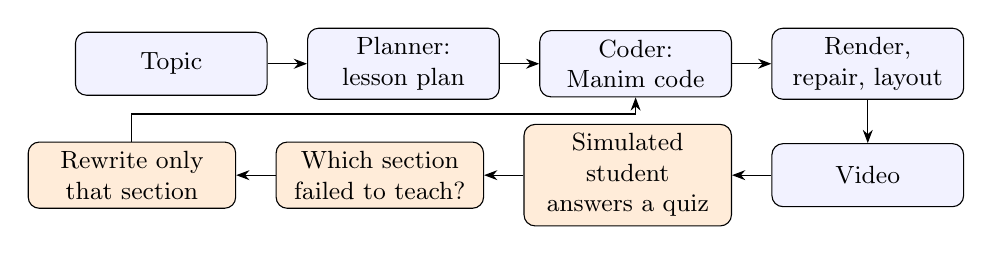
\begin{tikzpicture}[node distance=0.55cm and 0.5cm, every node/.style={font=\small},
  box/.style={draw, rounded corners, fill=blue!5, minimum height=0.8cm, align=center, text width=2.2cm},
  ours/.style={draw, rounded corners, fill=orange!15, minimum height=0.8cm, align=center, text width=2.4cm},
  >={Stealth}]
\node[box] (topic) {Topic};
\node[box, right=of topic] (plan) {Planner:\\lesson plan};
\node[box, right=of plan] (code) {Coder:\\Manim code};
\node[box, right=of code] (render) {Render,\\repair, layout};
\node[box, below=of render] (video) {Video};
\node[ours, left=of video] (student) {Simulated student\\answers a quiz};
\node[ours, left=of student] (diag) {Which section\\failed to teach?};
\node[ours, left=of diag] (fix) {Rewrite only\\that section};
\draw[->] (topic) -- (plan); \draw[->] (plan) -- (code); \draw[->] (code) -- (render); \draw[->] (render) -- (video);
\draw[->] (video) -- (student); \draw[->] (student) -- (diag); \draw[->] (diag) -- (fix);
\draw[->] (fix.north) |- ++(0,0.35) -| (code.south);
\end{tikzpicture}
\caption{The pipeline. Blue: the generation steps that earlier work built. Orange: the learner-feedback loop we
add.}\label{fig:pipeline}
\end{figure}

\subsection{The question: how do you know the video teaches?}

Rendering without errors and having a clean layout do not mean a video teaches. The honest test would be to show the
video to real students and quiz them, but that is slow, costly and impossible to repeat for every version of every
video. So recent work uses a \emph{simulated student}: a vision--language model that ``watches'' the video and
answers a multiple-choice quiz about the topic.

The catch is obvious once said: a large language model has read most of the internet. It already knows what a
determinant is. If it answers the quiz correctly after watching, did the video teach it, or did it know already?
Every result in this report comes back to this question.

\subsection{Our idea}

If a simulated student can tell us whether a video teaches, it can also tell us \emph{where} it fails to teach. Our
idea, called \textbf{learner-feedback repair}, is to (1) let the student take a practice quiz with the video, (2)
trace each question it fails to the section of the video that should have taught it, and (3) rewrite only that
section. The claim we want to test is narrow: \emph{a repair guided by the student's failures improves teaching on
new questions, written by other people, more than an equally large repair without that guidance.}

\begin{inshort}
Teaching videos can be generated as code. To improve them we use a simulated student's failures to find and fix the
weak section. To know whether that works, we must first be able to measure ``the video taught something'', and that
turned out to be the hard part.
\end{inshort}

%=====================================================================================================================
\section{Earlier work and what it leaves open}

\subsection{Code2Video and TeachQuiz}

Code2Video~\cite{code2video} is the closest earlier system. It builds the pipeline of Figure~\ref{fig:pipeline} (its
code repair, \emph{ScopeRefine}, fixes the failing line first, then a block around it, then the whole scene), and it
introduces two things we use:
\begin{itemize}
  \item \textbf{MMMC}, a benchmark of 117 topics taken from 3Blue1Brown lessons, each with 5 multiple-choice questions.
  \item \textbf{TeachQuiz}, its measure of teaching. A strong vision--language model (Gemini) gets a system prompt
  that tells it to \emph{forget} the topic: it may only use what the video shows, and it must answer \texttt{NULL}
  (``insufficient evidence'') when the video does not show the answer. It answers the quiz twice, without the video
  (score $S_1$) and with it ($S_2$). TeachQuiz is the difference $S_2 - S_1$.
\end{itemize}

\begin{example}[: how TeachQuiz is meant to work]
Question: ``What does the determinant of a $2\times2$ matrix measure?'' Without the video, the forgetful student
should answer \texttt{NULL}. After a video that shows a unit square being stretched into a parallelogram whose area
equals the determinant, it should answer ``the factor by which areas are scaled''. That change from \texttt{NULL}
to the right answer counts as teaching.
\end{example}

\DiagTeachQuiz
\imageslot{forget.png}{P2}{The idea behind TeachQuiz: a student told to forget, so that only the video can teach it.}

\textbf{What it leaves open.} TeachQuiz scores finished videos; it is not used to change them. And it relies on the
model actually forgetting when told to. Nobody had checked whether it does. (\hyperref[sec:refuse]{Breaks 2 and 3} shows that it
does not.)

\subsection{SGA: layout without rendering}

SGA~\cite{sga} runs a scene's code without drawing it, records the position and size of every object after every
animation (a \emph{scene graph}), and scores the layout with \textbf{MVQS}: overlaps, objects off the screen, text
too close together. It can tell the coder which object to move and in which direction. \textbf{What it leaves
open:} a perfect layout can still teach nothing; SGA does not measure learning.

\subsection{Other work}

\begin{center}\small
\begin{tabular}{p{2.6cm}p{5.4cm}p{6.4cm}}
\toprule
Work & What it does & What it leaves open for us \\
\midrule
ManimCode~\cite{manimcode} & makes generated Manim code render more often & render success, not teaching \\
EduPanel~\cite{edupanel} & a panel of models judges a teaching video & opinions about a video, not learning from it \\
PIVOT~\cite{pivot} & links quizzes to generated videos; a wrong answer makes a new remedial video for that learner &
fixes the learner, not the video; no link from a wrong answer to a part of the video \\
He-Yueya et al.~\cite{heyueya2024} & improves text worksheets using simulated learning gains & text, not video; no
localisation \\
VideoMathQA~\cite{videomathqa} & shows models answer video maths questions from text and narration, skipping the
visuals & a warning about shortcuts, not a teaching measure \\
TOFU~\cite{tofu} & tests ``forgetting'' on \emph{invented} authors, because real knowledge cannot be controlled & the
idea we borrow for NOVEL-12 \\
\bottomrule
\end{tabular}
\end{center}

\begin{inshort}
Earlier work can generate the video, repair its code and its layout, and score how much a simulated student learns.
No one had used the student's failures to repair the video, and no one had checked whether the student really forgets
what it is told to forget.
\end{inshort}

%=====================================================================================================================
\section{How we set up the test}\label{sec:setup}

\subsection{Two quizzes that never mix}

A repair that looks at a quiz can simply teach that quiz's questions. To prevent this, every topic has two quizzes:
\begin{itemize}
  \item \textbf{DEV} (practice): written by our own planner. The repair may look at it.
  \item \textbf{TEST} (final exam): written by \emph{other people} (MMMC's official questions). No step of the
  pipeline ever sees it. All results are on TEST.
\end{itemize}

\DiagDevTest

\subsection{Three ways to rewrite, so the comparison is fair}

Rewriting a video might help just because it was rewritten. So we compare three conditions that use the same first
video and the same diagnosis:
\begin{itemize}
  \item \textbf{learner} (ours): rewrite the sections the diagnosis blames, telling the coder what idea was missing;
  \item \textbf{generic}: rewrite the \emph{same number} of sections, chosen at random, with ``teach this more
  clearly'';
  \item \textbf{learner\_all}: rewrite \emph{every} section with all the missing ideas.
\end{itemize}
If learner beats generic, the student's signal matters (same amount of rewriting). If learner beats learner\_all,
\emph{where} you fix matters too.

\subsection{Which model does what}

All models run locally (Ollama). Table~\ref{tab:models} lists the model behind every part. Three choices matter.
\begin{itemize}
  \item \textbf{The student and the judge come from different families} (\texttt{gemma4:26b} and
  \texttt{qwen2.5vl:7b}), so the judge is less likely to share the student's weak spots. We did not test this.
  \item \textbf{The NOVEL-12 final quiz is written by a family the pipeline never uses} (Claude). The numeric answers
  are computed by code.
  \item \textbf{Several parts use no model at all:} the code check, the layout score, the weak-section score and the
  gate. Their behaviour is fixed and can be checked by reading the code.
\end{itemize}

\begin{table*}[t]\centering\footnotesize
\caption{Which model does each part. Every model runs locally through Ollama, except the authors of the final quizzes. The student and the judge come from different families; the NOVEL-12 final quiz is written by a family the pipeline never uses.}\label{tab:models}
\begin{tabular}{@{}lp{9.2cm}l@{}}\toprule Part & What it does & Model\\
\midrule
\multicolumn{3}{c}{\textit{Making the video (every step and stage)}}\\
Planner & lesson plan: what each section teaches, shows and says & \texttt{qwen3.6:latest} \\
Coder & one Manim scene per section; render repairs (line, block, section) & \texttt{qwen3-coder:30b} \\
Code check (F2) & reads the code and the installed Manim library before rendering & \textit{no model} \\
Timing check (F2) & leftovers after Transform, prose typeset as maths; fixed automatically & \textit{no model} \\
Admission & all sections render, layout at least 70, a person approves the frames & \textit{no model} \\
Layout check & SGA scene graph and MVQS; the coder writes the fixes & \textit{no model}; \texttt{qwen3-coder:30b} \\
\midrule
\multicolumn{3}{c}{\textit{Learner feedback (the repair)}}\\
Practice quiz (DEV) & written from the topic, or from the card of an invented concept & \texttt{qwen3.6:latest} \\
Practice-quiz check & keeps questions the student solves with the card and not without the video & \texttt{gemma4:26b} \\
Diagnosis & the missing idea of each failed question; question-to-section map (F3) & \texttt{qwen3.6:latest} \\
Weak-section score (F3) & Ochiai score from passed and failed practice questions & \textit{no model} \\
Leak guard (F4) & refuses fixes that copy the practice question; merges ideas into one & rules; \texttt{qwen3.6:latest} \\
Small edit (F5) & edits the working scene instead of rewriting it & \texttt{qwen3-coder:30b} \\
Gate (F1) & practice score must not drop; layout must fall by less than 5 & \textit{no model} \\
\midrule
\multicolumn{3}{c}{\textit{Measuring}}\\
Student & TeachQuiz, forced choice, D-VGAIN, practice scores (Steps 0--3) & \texttt{gemma4:26b} \\
Evidence judge & does a frame show the answer (TeachQuiz pilot only) & \texttt{qwen2.5vl:7b} \\
Second student & what a different family knows with no video (Step 0) & \texttt{qwen2.5vl:7b} \\
Small student & MMMC ladder with a 3B model (Step 1) & \texttt{qwen2.5vl:3b} \\
\midrule
\multicolumn{3}{c}{\textit{Final quizzes (TEST), never seen by the pipeline}}\\
MMMC & Code2Video's official questions, 5 per topic & Code2Video \\
NOVEL-12 & cards and 8 questions per concept; numeric answers computed by code & Claude (Anthropic) \\
\midrule
\multicolumn{3}{c}{\textit{Layout reference (side study on the 10 admitted videos)}}\\
Claude fixer & repairs layout and timing only; sees code, frames and reports, never the plan, card or quiz & \texttt{claude-opus-5-5} \\
\midrule
\multicolumn{3}{c}{\textit{Reference, not run here}}\\
Code2Video's student & watches the video file with sound (needs a paid key) & Gemini \\
\bottomrule\end{tabular}
\end{table*}


\subsection{How we decide}

As in Code2Video, every score is on a 0--100 scale and every table shows one number per cell: the mean over the 12
topics. A comparison such as ``learner $-$ base'' is the mean, over topics, of the learner video's score minus the base
video's score; above 0 favours the learner repair. We also count \emph{ties}: topics where both videos score the same,
which tell us nothing about which is better. (Statistical checks over topics are kept with the result files.)

%=====================================================================================================================
\section{The study, step by step}

The study has four steps, and each one explains the next (Figure~\ref{fig:study-flow}).
\begin{itemize}
  \item \textbf{Step 0, pilot and audit.} We ran the repair on 12 MMMC topics, saw no effect, and looked for the
  reason. We found three breaks in the measure, not only in the method. \emph{Models:} \texttt{qwen3.6} plans,
  \texttt{qwen3-coder:30b} codes, \texttt{gemma4:26b} is the student, \texttt{qwen2.5vl:7b} judges the evidence
  and is the second student for the no-video check.
  \item \textbf{Step 1, the metric ladder on MMMC.} We rebuild the measure one change at a time (M0 to M9) and test
  every version on the pilot's videos, with our student and with a smaller one. \emph{Models:} students
  \texttt{gemma4:26b} and \texttt{qwen2.5vl:3b}; no video is generated in this step.
  \item \textbf{Step 2, the metric ladder on NOVEL-12.} We repeat the ladder on invented concepts that no model has
  seen, and fix the measure for Step 3: the gain on 3 frames per section (M9), with the full D-VGAIN on the dense video (M7)
  as a second measure. \emph{Models:} the same generator and student
  as Step 0; the cards and the final quiz are written by Claude, with answers computed by code.
  \item \textbf{Step 3, the pipeline features F0 to F5.} We add one feature at a time to the repair loop, the gate
  first, and score every stage with M9 and M7. \emph{Models:} \texttt{qwen3.6} diagnoses, maps questions
  to sections and merges ideas; \texttt{qwen3-coder:30b} rewrites or edits; \texttt{gemma4:26b} scores the practice
  quiz and the final quiz.
\end{itemize}

\textbf{How a version of the measure is judged.} Every version on the ladder faces the same four tests on the same
videos:
\begin{enumerate}
  \item does it give a score at all;
  \item does a topic's own video score higher than another topic's video on the same quiz, which is the core check
  that it measures the video;
  \item do two measurements of the same videos agree;
  \item how many repaired videos tie with their base video.
\end{enumerate}
These tests and the decision rules of Section~\ref{sec:results-long} were fixed before the NOVEL-12 results existed.

\DiagStudy

\subsection{Step 0: the pilot and the audit}

This step is the history of the first runs: what we tried, what came out, and the three breaks we found.

\subsubsection*{The first single topic}

We first ran the whole loop on one topic (Pythagoras' theorem). The learner repair scored slightly higher than the
generic one. One topic is an anecdote, not evidence. But the run exposed problems that we fixed before going further:
\begin{itemize}
  \item practice questions the student could answer with no video at all (now filtered out);
  \item a small judge model, asked to judge a list, copied the example ids from the instructions, so every ``yes'' was
  lost (now one question per call; remember this pattern, it returns in \hyperref[sec:idbug]{Break 1});
  \item a rewrite that failed to render deleted its section (now the old section is kept);
  \item Manim's error message hides the failing line (now taken from SGA-style partial execution).
\end{itemize}

\subsubsection*{The pilot on 12 MMMC topics, and no signal}

We then ran the full protocol on 12 MMMC topics (Table~\ref{tab:pilot}). The learner repair beat the base video by only a
point or two, and \PilotTies{} of 12 topics were exact ties, most of them at a TeachQuiz of 0.

\begin{table}[t]\centering\small
\caption{Pilot on 12 MMMC topics, scored with TeachQuiz as in Code2Video (local student, 3 frames per section, graded as in the pilot, before the fix of Break 1; the regraded score is version M1 of the ladder). TeachQuiz: quiz score with the video minus without it. Evidence: answers a judge could find in the frames. Layout: SGA's MVQS. Small numbers: change against the base video.}\label{tab:pilot}
\begin{tabular}{lrrrr}\toprule Method & TeachQuiz ($\uparrow$) & Evidence ($\uparrow$) & Layout ($\uparrow$) & Sections rendered ($\uparrow$)\\
\midrule
\multicolumn{5}{c}{\textit{Repair of the base video}}\\
Base video (first attempt) & 10.6 & 7.8 & 78.5 & 3.25 \\
Generic repair & 14.4\better{+3.9} & 6.7 & 79.2 & 3.58 \\
Learner repair, every section & 16.7\better{+6.1} & 11.1 & 72.6 & 3.50 \\
Learner repair (ours) & 12.2\better{+1.7} & 8.9 & 79.3 & 3.67 \\
\bottomrule\end{tabular}
\end{table}

\datafig{pilot}{The pilot, topic by topic: TeachQuiz for the four conditions (graded before the fix of \hyperref[sec:idbug]{Break 1}). Most
points sit at 0 in every condition; a tie at 0 says nothing about which repair is better.}

\subsubsection*{Listing what breaks}\phantomsection\label{sec:breaks}

We measured every part of the pilot to see why. Four problems stood out. They are symptoms; the three breaks in the measure that explain most of them follow in \hyperref[sec:idbug]{Breaks 1--3}.
\begin{enumerate}
  \item \textbf{Floor.} Most videos scored 0 in every condition. With 5 questions a topic, one question is worth 20
  points; a tie at 0 carries no information.
  \item \textbf{Localisation never happened.} The diagnosis called \PilotGaps{} of \PilotDev{} practice questions
  ``gaps'', meaning questions the student did not learn from the video. It flagged on average \PilotFlagged{} of \PilotSections{} sections. ``Fix only the weak section'' became
  ``fix almost everything'', the same as learner\_all. We call this \emph{localisation collapse}.
  \item \textbf{Practice gains did not carry over.} The learner repair raised its own DEV score by \PilotDevGain{}
  points on average, while TEST did not move. Either the repair taught the practice questions, or something made DEV
  and TEST behave differently (\hyperref[sec:idbug]{Break 1} found the second).
  \item \textbf{Code that does not run.} \FirstTryFail\% of sections failed to render on the first try. The
  pilot's \FailedAttempts{} failed attempts are broken down in Table~\ref{tab:failures}; \SyntaxAfterPatch{} of them
  were syntax errors that \emph{our own} repair created when it pasted a fixed line back into the file.
  A rewrite that never renders leaves the old section in place, so conditions differ less than intended.
\end{enumerate}

\begin{table}[t]\centering\small
\caption{Failed render attempts in the pilot (12 MMMC topics, base and revised videos), by class. Pre-flight raises an alarm on 1 of 156 sections that rendered.}\label{tab:failures}
\begin{tabular}{lr}\toprule Class & Attempts\\\midrule
unknown keyword / method & 69 \\
undefined name & 41 \\
syntax / indentation & 39 \\
\quad of which right after a patch & 38 \\
other & 36 \\
external file or URL & 22 \\
2-D point where 3-D needed & 20 \\
LaTeX & 14 \\
\bottomrule\end{tabular}
\end{table}

\datafig[0.75]{failures}{Why generated code fails to render (pilot). The orange part of the syntax bar was created by
our own repair pasting a fixed line back into the file.}

\subsubsection*{Break 1: a grading bug}\phantomsection\label{sec:idbug}

To test whether the floor came from the student, we re-scored the pilot's videos with variants of the student. The
scores came back strangely all-or-nothing: a run was either fully right or fully \texttt{NULL}. Reading the raw
replies showed why. The answer template in the prompt shows an example answer with id \texttt{q1}. MMMC's TEST
questions are named \texttt{t1} to \texttt{t5}. The student often wrote its answers as \texttt{q1..q5}, and the grader,
matching answers to questions by id, found none: every answer of that run was scored \texttt{NULL}. This happened in
\OrderRuns{} of \AllRuns{} graded runs (\OrderShare\%).

\DiagIdBug

It explains problem 3 in the \hyperref[sec:breaks]{list of problems}. DEV questions are named \texttt{q1..} like the template, so DEV was never affected:
the bug alone made DEV look better than TEST. We fixed it by matching answers in order when no id matches. Every
TEST number from the pilot had to be measured again; the student-variant study was stopped and replaced.

\subsubsection*{Breaks 2 and 3: the student refuses, and it already knows}\phantomsection\label{sec:refuse}

Graded correctly, the student still answered \texttt{NULL} on \NullNoVideo\% of questions without the video and on
\NullWithVideo\% with it. When it did answer with the video, it was right \AnsweredRight{} times out of
\AnsweredWithVideo{}: it answered only what it already knew. So we asked a simple question: what if the student is not allowed to say \texttt{NULL}? We
kept Code2Video's ``forget this topic'' prompt word for word, removed the \texttt{NULL} option, showed it
\emph{nothing}, and asked every one of MMMC's questions (Table~\ref{tab:priors}).

\begin{table*}[t]\centering\small
\caption{What the student already knows. Code2Video's unlearning prompt, but the student must choose A--D (no NULL). Accuracy: share of questions right. Confidence: mean probability the student puts on the right answer. Fully known: topics where every question is right with no video. Chance is 25.}\label{tab:priors}
\begin{tabular}{llrrrrr}\toprule Material & Student & Topics & Questions & Accuracy (\%) & Confidence (\%) & Fully known\\
\midrule
\multicolumn{7}{c}{\textit{MMMC (real topics from 3Blue1Brown)}}\\
No video & gemma4:26b & 117 & 585 & 99.0 & 99.0 & 108 \\
No video & qwen2.5vl:7b & 117 & 585 & 97.4 & 95.6 & 99 \\
No video & qwen2.5vl:3b & 117 & 585 & 91.9 & 86.6 & 67 \\
\midrule
\multicolumn{7}{c}{\textit{NOVEL-12 (invented concepts)}}\\
No video & gemma4:26b & 12 & 96 & 41.1 & 41.4 & 0 \\
Definition card as text & gemma4:26b & 12 & 96 & 84.9 & 83.7 & 1 \\
\bottomrule\end{tabular}
\end{table*}

\datafig{refusal}{What the student's answers are. Under TeachQuiz it refuses almost everything; when it does answer
with the video, it is almost never wrong, which is what one expects when the answers come from what it already
knew. Forced to choose with no video, it is right on most MMMC questions.}
\datafig{priors}{Per question, the probability the student without the video puts on the right answer. On MMMC almost every
question sits at 1 (already known). On NOVEL-12 the questions spread out, and the card (the ideal lesson) moves them
to the right.}
\imageslot{refuse.png}{P3}{Refusing is not forgetting: the student says ``insufficient evidence'' while it knows the
answer.}
\imageslot{knows.png}{P4}{The prior ceiling: on MMMC the student knows the answers before the video starts.}

The student, supposedly ignorant, answered \mmmcpriorGemmaAcc\% of MMMC's questions correctly with no video at all,
and was nearly certain each time (average confidence in the right answer \mmmcpriorGemmaP\%). Smaller models did
the same: \mmmcpriorQwenAcc\% for a 7B model and \mmmcpriorQwenSmallAcc\% for a 3B model. We checked that this is not a preference for some letter: when the options are
shifted (the text of A moves to B, and so on) the student follows the right text.

\begin{inshort}
TeachQuiz's ``before'' score of 0 was never ignorance. The student refused to answer what it knew (\emph{refusal}). Its ``after''
score measured when the video made it willing to answer, and on MMMC the answers were already known (a \emph{prior
ceiling}). No change to
the scoring can show learning on questions the student already knows.
\end{inshort}

\paperfig{fig_failures.png}{F3}{\textbf{Why TeachQuiz cannot see teaching on MMMC.} (i) The grader lost answers whose ids copied the prompt's
template. (ii) The student refuses instead of forgetting. (iii) It already knows the answers. Bottom: our fix for
each.}{failures3}

\subsection{Step 1: a new measure, built one change at a time and tested on MMMC}

D-VGAIN (Dynamic Video-Grounded Gain) was proposed in our discussions to replace TeachQuiz. Its parts, each
answering one problem above:
\begin{itemize}
  \item \textbf{No \texttt{NULL}.} The student must choose. A refusal can no longer pass as ignorance.
  \item \textbf{Measure the prior instead of asking to forget it.} $\Sblind$ is the score with no video. With 4
  options, chance is $c = 0.25$, and the baseline is $\Beff = \max(c, \Sblind)$.
  \item \textbf{Normalised gain} (Hake's $g$~\cite{hake1998}, from physics education): how much of the room left
  above the baseline the video filled,
  \[ \mathrm{NVG} = \frac{S - \Beff}{1 - \Beff}. \]
  A student who already knows everything leaves no room, and NVG is then \emph{undefined}, not 0.
  \item \textbf{A silent, dense video.} $\Svisual$ uses up to 4 frames a second of the muted video, so the student
  must read the animation, not a narration.
  \item \textbf{A motion control.} $\Sstatic$ shows only the first and last frame of each section: a slide deck of
  start and end states. $\mathrm{DML} = \Svisual - \Sstatic$ is what the animation adds. The full measure is
  $\text{D-VGAIN} = \mathrm{NVG}(\Svisual) + 0.5 \max(0, \mathrm{DML})$.
  \item \textbf{Continuous scores.} Instead of right/wrong, read the probability the student puts on the right letter,
  so a video that raises confidence from 25\% to 45\% counts even if the top answer does not change.
  \item \textbf{Option rotation.} Ask twice with the options shifted, and average, so a liking for one letter cancels.
\end{itemize}

\paragraph{What we changed from the proposal, and why.}
\begin{itemize}
  \item \emph{One letter per call did not work}: the student's first word was often not a letter, and one call per
  question with 400 frames took 90 seconds. The student now answers all questions in one reply (``\texttt{1: B}'' per
  line) and we read the probabilities at each letter.
  \item \emph{Forced choice still refused sometimes}: the student wrote an explanation of why it could not answer.
  Such replies are asked again (at most twice) with a stricter line.
  \item \emph{The normalised gain explodes near the prior ceiling}: with continuous scores, a no-video probability of
  0.99999 leaves 0.00001 of room, and dividing by it turned tiny noise into ``gains'' of $\pm 10$ on a scale meant to
  run from $-1$ to $1$. NVG is now undefined when less than 0.05 of room is left.
  \item \emph{Pooling questions across topics was not used}: a video is made per topic, so the topic, not the
  question, is what receives a treatment; pooling 60 questions would pretend there are 60 independent experiments.
  \item \emph{Multiplying by the evidence judge was not used}: the judge can only check answered questions, so
  multiplying by it brings back the refusal floor.
\end{itemize}

\DiagDVGAIN
\paperfig{fig_measure.png}{F4}{\textbf{How we measure.} The same student, without NULL, answers the quiz from four materials. We read its
confidence in each letter, average two option orders, and report the gain over what it knew with no video.}{measure}

\paragraph{The ladder.} To see which part matters, we add the parts one at a time, M0 to M9, and judge every version by
the same four tests on the same videos: is the score \emph{defined}; does a topic's own video beat \emph{another
topic's video} (if it does not, the measure cannot be measuring teaching); is it \emph{reliable} (two measurements
agree); and does it \emph{resolve} differences (few ties). Table~\ref{tab:ladder_mmmc} is the ladder on the pilot's
videos.

\DiagLadder
\begin{table*}[t]\centering\footnotesize
\caption{Metric ladder on the MMMC pilot videos. 12 topics, 48 videos. Each row adds one change to the row above; points on a 0--100 scale. Scored: videos that get a score (-- : the student already knew everything). Own $-$ other: a topic's video minus another topic's video on the same quiz. Agreement: rank correlation of two measurements of the same videos. Learner $-$ \ldots: mean change over topics. Ties: topics where learner and base score the same.}\label{tab:ladder_mmmc}
\setlength{\tabcolsep}{4pt}\begin{tabular}{@{}llrrrrrrr@{}}\toprule & & \multicolumn{3}{c}{Does it measure teaching?} & \multicolumn{4}{c}{Does the learner repair help?}\\
\cmidrule(lr){3-5}\cmidrule(lr){6-9}
& Measure & Scored & \hd{Own $-$\\other ($\uparrow$)} & \hd{Agree-\\ment ($\uparrow$)} & \hd{Learner\\$-$ base} & \hd{Learner\\$-$ generic} & \hd{Learner $-$\\every section} & Ties ($\downarrow$)\\\midrule
M0 & TeachQuiz (Code2Video) & 48/48 & +10.6 & -- & +1.7 & $-$2.2 & $-$4.5 & 7/12 \\
M1 & + answers matched in order & 47/48 & +10.6 & 0.96 & +7.2 & +2.8 & +0.6 & 7/12 \\
M2 & + must choose (no NULL) & 48/48 & +16.7 & 1.00 & 0.0 & 0.0 & 0.0 & 12/12 \\
M3 & + gain over what it knew & 0/48 & -- & -- & -- & -- & -- & -- \\
M4 & + dense silent video & 0/48 & -- & -- & -- & -- & -- & -- \\
M5 & + motion bonus (D-VGAIN) & 0/48 & -- & -- & -- & -- & -- & -- \\
M6 & + confidence, not right/wrong & 0/48 & -- & -- & -- & -- & -- & -- \\
M7 & + two option orders & 0/48 & -- & -- & -- & -- & -- & -- \\
M8 & + only questions it did not know & 0/48 & -- & -- & -- & -- & -- & -- \\
M9 & M7 on 3 frames per section & 0/48 & -- & -- & -- & -- & -- & -- \\
\midrule
\multicolumn{9}{c}{\textit{Raw difference in confidence, not normalised (for reference)}}\\
R7 & Dense video minus no video & 48/48 & +4.1 & 0.65 & +1.4 & $-$0.1 & +0.3 & 1/12 \\
R9 & 3 frames minus no video & 48/48 & +13.0 & 0.77 & +0.1 & 0.0 & +0.1 & 0/12 \\
\bottomrule\end{tabular}
\end{table*}

\datafig{ladder_mmmc}{The ladder on the MMMC pilot videos. Left: does a topic's own video beat another topic's video
(mean difference in points)? Right: for how many videos the measure gives a score at all.}

\paragraph{A smaller student.} If the student knows less, does the measure come alive on MMMC? A 3B model
(\texttt{qwen2.5vl:3b}) still answers \mmmcpriorQwenSmallAcc\% of all MMMC questions with no video. On the 12 pilot
topics its confidence in the right answer with no video is \LadSmallSBlind{}, so the gain on 3 frames per section (M9)
now scores \LadSmallDefinedNine{} videos (Table~\ref{tab:ladder_small}). Our analysis yields two insights.
(i) \textbf{The measure sees the video.} A topic's own video beats another topic's video by \LadSmallSepNine{} points
(raw confidence: \LadSmallSepRawNine{}).
(ii) \textbf{It still cannot see the repair.} The learner repair scores \LadSmallLBNine{} points against the base video
(raw: \LadSmallLBRawNine{}) and \LadSmallLGNine{} against the generic repair. With so little room left, each topic's
gain rests on one or two questions, and one question can move it by tens of points. Even for a small student, MMMC
is a poor test of repair; NOVEL-12 leaves far more room.

\begin{table*}[t]\centering\footnotesize
\caption{A smaller student (qwen2.5vl:3b) on the MMMC pilot videos, 3 frames per section only; measures it could not score are left out. 12 topics, 48 videos. Each row adds one change to the row above; points on a 0--100 scale. Scored: videos that get a score (-- : the student already knew everything). Own $-$ other: a topic's video minus another topic's video on the same quiz. Agreement: rank correlation of two measurements of the same videos. Learner $-$ \ldots: mean change over topics. Ties: topics where learner and base score the same.}\label{tab:ladder_small}
\setlength{\tabcolsep}{4pt}\begin{tabular}{@{}llrrrrrrr@{}}\toprule & & \multicolumn{3}{c}{Does it measure teaching?} & \multicolumn{4}{c}{Does the learner repair help?}\\
\cmidrule(lr){3-5}\cmidrule(lr){6-9}
& Measure & Scored & \hd{Own $-$\\other ($\uparrow$)} & \hd{Agree-\\ment ($\uparrow$)} & \hd{Learner\\$-$ base} & \hd{Learner\\$-$ generic} & \hd{Learner $-$\\every section} & Ties ($\downarrow$)\\\midrule
M0 & TeachQuiz (Code2Video) & 48/48 & -- & -- & +1.7 & $-$2.2 & $-$4.5 & 7/12 \\
M2 & + must choose (no NULL) & 48/48 & +10.0 & 0.65 & $-$3.3 & +1.7 & +3.3 & 9/12 \\
M3 & + gain over what it knew & 24/48 & +16.7 & 0.72 & +25.0 & +8.3 & +16.7 & 4/12 \\
M9 & M7 on 3 frames per section & 36/48 & +37.9 & -- & $-$23.7 & $-$0.6 & +5.9 & 1/12 \\
R9 & 3 frames minus no video & 48/48 & +6.4 & 0.70 & $-$2.9 & +0.2 & +1.2 & 1/12 \\
\bottomrule\end{tabular}
\end{table*}


\subsection{Step 2: concepts the student cannot already know (NOVEL-12)}

If the student knows the answers, nothing can measure learning. So we made topics that no model has seen. Following
TOFU's invented authors~\cite{tofu}, we wrote 12 small \emph{invented} mathematical concepts. Each has a \emph{card}:
a definition, three or four rules and a worked example (all cards are in Appendix~\ref{app:cards}).

\begin{example}[: an invented concept]
\textbf{Tovan sum.} $a \oplus b = a + b + a \times b$. Rules: order does not matter; 0 is neutral; $-1$ swallows
everything. Worked example: $2 \oplus 3 = 2 + 3 + 6 = 11$.
A TEST question: ``What is $1 \oplus 4$?'' A) 5, B) 9, C) 4, D) 10. No model has seen this definition, so to answer B
it must learn the rule from the video.
\end{example}

The planner, coder and practice-quiz writer are given the card, because otherwise they could not write about the
topic. TEST (8 questions per concept, 96 in all) was written from the cards by a different model family that the
pipeline never uses, and the correct answers to computation questions were calculated by code. So the arithmetic in
the key is checked by construction; no teacher has reviewed the questions yet. The right letters are spread evenly (24 each of A to D).

\textbf{Checks that the benchmark works.} Without the video, the student scores \novelpriorGemmaAcc\% (25\% is pure guessing;
on MMMC it was \mmmcpriorGemmaAcc\%). Given the card as plain text, the ideal lesson, it scores
\novelcardGemmaAcc\%. So a video has room to show teaching, between about \novelpriorGemmaAcc\% and
\novelcardGemmaAcc\%. We checked every question the student misses even with the card: in each case the key is right
and the student made an arithmetic slip. Some questions can be guessed from their wording (``is $a \oplus b$ the same
as $b \oplus a$?''); the baseline $\Beff$ and version M8 (only questions the student does not know beforehand) take
care of them.

\imageslot{invented.png}{P5}{Invented concepts: new mathematics that no model has seen, so only the lesson can
teach it.}
\paperfig{fig_novel.png}{F5}{\textbf{NOVEL-12.} Twelve invented concepts, each defined on one card, with 96 TEST questions. Without the video, the
student is close to chance; the card shows how much a perfect lesson could teach.}{novelfig}

\subsubsection*{First look: do the pipeline's videos teach invented concepts?}

Table~\ref{tab:novel_first} and Figure~\ref{fig:novel_first} show the NOVEL-12 base videos measured so far, before any
repair. Not all 12 are in yet; the Mean row is over the concepts listed. Table~\ref{tab:novel_items} takes one concept question by question. Two things are already visible.

\textbf{The frames teach what the student could not know.} Take computation questions that the student without the video
gets wrong, such as the value of a tovan sum. With 3 frames per section, the probability on the right answer rises on
several of them (Table~\ref{tab:novel_items}). The dense video helps less. These are questions it cannot have known before: this is the signal MMMC could never show. The
questions it already got right without the video are the guessable ones (``does order matter?''), and they stay right.

\textbf{How the video is shown matters.} TeachQuiz's material, three sharp frames per section, taught at least as
much as the dense silent video of up to 4 frames a second, and on one concept far more. A local student sees each
dense frame at low resolution (about 70 tokens) among hundreds of others, and seems to lose the on-screen text. This
is why version M9 measures the gain on the three-frame material; the full ladder (Table~\ref{tab:ladder_novel}) will show
over all 12 concepts whether the dense video helps, hurts or does not matter.

\begin{table*}[t]\centering\footnotesize\setlength{\tabcolsep}{4pt}
\caption{NOVEL-12 base videos (the pipeline's first attempt, before any repair). Confidence: mean probability on the right answer over 8 TEST questions and two option orders, in \%; chance is 25. TeachQuiz: Code2Video's measure on the same video. Gain: share of what the student did not know that the video taught (100 = all of it), from 3 frames per section (M9) or the same gain on the dense video; D-VGAIN (M7) adds the motion bonus to the dense-video gain.}\label{tab:novel_first}
\begin{tabular}{lrrrrrrrr}\toprule & \multicolumn{4}{c}{Confidence on the right answer} & & \multicolumn{3}{c}{Ours ($\uparrow$)}\\
\cmidrule(lr){2-5}\cmidrule(lr){7-9}
Concept & No video & 3 frames & Start/end & Dense video & TeachQuiz & Gain, 3 frames & Gain, dense & D-VGAIN\\\midrule
Tovan sums & 50.6 & 88.4 & 47.7 & 56.3 & +33.3 & +76.4 & +11.5 & +15.8 \\
Krell steps on a grid & 20.0 & 44.3 & 27.7 & 38.6 & +50.0 & +25.8 & +18.1 & +23.6 \\
Vorn sequences & 58.5 & 76.2 & 60.3 & 79.1 & +87.5 & +42.7 & +49.7 & +59.1 \\
Glint numbers & 43.9 & 88.3 & 38.9 & 52.8 & +62.5 & +79.2 & +15.9 & +22.8 \\
Mirthful triangles & 47.4 & 69.5 & 37.9 & 56.6 & +37.5 & +42.0 & +17.5 & +26.8 \\
Sorrel counts of lattice rectangles & 66.8 & 57.5 & 63.3 & 61.4 & +12.5 & $-$27.9 & $-$16.0 & $-$16.0 \\
Quill distance & 25.2 & 45.3 & 43.0 & 33.9 & +25.0 & +26.9 & +11.6 & +11.6 \\
Dapple numbers & 33.7 & 64.0 & 39.5 & 39.0 & +37.5 & +45.6 & +7.9 & +7.9 \\
Orbit words & 32.0 & 74.1 & 73.1 & 45.3 & +79.2 & +61.9 & +19.5 & +19.5 \\
Vells of 2×2 grids & 31.9 & 67.2 & 41.0 & 35.2 & +58.3 & +51.8 & +4.8 & +4.8 \\
\midrule
Mean & \textbf{41.0} & \textbf{67.5} & \textbf{47.2} & \textbf{49.8} & \textbf{+48.3} & \textbf{+42.4} & \textbf{+14.1} & \textbf{+17.6} \\
\bottomrule\end{tabular}
\end{table*}

\datafig[0.75]{novel_first}{NOVEL-12 videos measured so far: mean probability on the right answer with no video,
three frames per section, the first and last frame of each section, and the dense silent video. Dotted line:
chance.}
\begin{table*}[t]\centering\footnotesize
\caption{Tovan sums, question by question: the student's confidence in the right answer (\%, mean of two option orders) under each material. The video is the pipeline's first attempt, before any repair.}\label{tab:novel_items}
\begin{tabular}{p{6.4cm}p{2.4cm}rrrr}\toprule Question & Answer & No video & 3 frames & Start/end & Dense video\\\midrule
What is 1 ⊕ 4 (tovan sum)? & 9 & 5 & 100 & 9 & 7 \\
What is 3 ⊕ 3? & 15 & 0 & 50 & 0 & 0 \\
Which number is neutral for the tovan sum (n ⊕ b = b for every b)? & 0 & 100 & 100 & 53 & 94 \\
What is (-1) ⊕ 9? & -1 & 0 & 57 & 0 & 1 \\
What is 2 ⊕ 2 ⊕ 2, worked left to right? & 26 & 4 & 100 & 20 & 62 \\
Is 5 ⊕ 7 equal to 7 ⊕ 5? & Yes, always & 96 & 100 & 99 & 99 \\
What is 0 ⊕ 6? & 6 & 100 & 100 & 100 & 100 \\
A student says 2 ⊕ 3 = 5. What did they forget? & To add the product 2×3 & 100 & 100 & 99 & 88 \\
\bottomrule\end{tabular}
\end{table*}


\paragraph{The ladder on the admitted NOVEL-12 videos.} Table~\ref{tab:ladder_novel} repeats the ladder on the
\LadNovelTopics{} concepts whose videos passed admission (next section), on their base videos. The repairs are not
measured here; that is Step~3. Four things stand out.

\textbf{Where the student has room to learn, every version gives a score.} Without the video, its confidence on the
right answer is \LadNovelSBlind{}. Every version from M1 on scores all \LadNovelVideos{} videos. On MMMC, the gain
versions scored none.

\textbf{A topic's own video beats another topic's video by a wide margin.} With the gain on 3 frames per section (M9),
the own video is \LadNovelSepNine{} points ahead. With the full D-VGAIN on the dense video (M7: with confidence and
both option orders), it is \LadNovelSepSeven{} points ahead.

\textbf{Even TeachQuiz separates the videos here, once its answers are matched in order.} M1 puts the own video
\LadNovelSepOne{} points ahead. This suggests that on MMMC the grading bug and the prior ceiling, more than the quiz
itself, hid the signal. We did not test this directly. Refusal has not gone away: with the video, the student still refused \LadNovelAbstained\% of
TeachQuiz questions (\NullWithVideo\% on MMMC).

\textbf{Three frames per section teach more than the dense video, and their scores repeat better.} Confidence on the
right answer is \LadNovelSFrames{} with 3 frames per section, \LadNovelSVisual{} with the dense video, and
\LadNovelSStatic{} with only the first and last frame of each section. We check whether a score repeats by measuring it
again with the answer options in a different order, and taking the rank correlation across the 10 concepts. For the
raw gain on 3 frames it is \LadNovelAgreeRawNine{}, which is modest. The dense-video versions barely agree with themselves (M4 to M6
and R7). This supports M9 as the main measure for Step~3. Two limits apply. M7 to M9 average both option orders, so
their agreement is not measured. And these are 10 concepts and one student.

\begin{table}[t]\centering\footnotesize
\caption{Metric ladder on NOVEL-12. 10 topics, base videos only (the repairs are future work). Each row adds one change to the row above; points on a 0--100 scale. Scored: videos that get a score. Own $-$ other: a topic's video minus another topic's video on the same quiz. Agreement: rank correlation of two measurements of the same videos.}\label{tab:ladder_novel}
\setlength{\tabcolsep}{4pt}\begin{tabular}{@{}llrrr@{}}\toprule & Measure & Scored & \hd{Own $-$\\other ($\uparrow$)} & \hd{Agree-\\ment ($\uparrow$)}\\\midrule
M0 & TeachQuiz (Code2Video) & 7/10 & -- & -- \\
M1 & + answers matched in order & 10/10 & +48.3 & 0.67 \\
M2 & + must choose (no NULL) & 10/10 & +42.5 & 0.21 \\
M3 & + gain over what it knew & 10/10 & +74.5 & 0.43 \\
M4 & + dense silent video & 10/10 & +30.7 & -0.19 \\
M5 & + motion bonus (D-VGAIN) & 10/10 & +32.5 & -0.07 \\
M6 & + confidence, not right/wrong & 10/10 & +23.7 & 0.10 \\
M7 & + two option orders & 10/10 & +26.5 & -- \\
M8 & + only questions it did not know & 10/10 & +26.5 & -- \\
M9 & M7 on 3 frames per section & 10/10 & +64.4 & -- \\
\midrule
\multicolumn{5}{c}{\textit{Raw difference in confidence, not normalised (for reference)}}\\
R7 & Dense video minus no video & 10/10 & +12.1 & -0.31 \\
R9 & 3 frames minus no video & 10/10 & +36.2 & 0.30 \\
\bottomrule\end{tabular}
\end{table}


\subsection{Step 2b: are the videos good enough to test?}\label{sec:quality}

Before measuring whether a repair improves a video, the video itself must be complete and readable. Looking at the
frames showed it often was not.

\paragraph{Admission.} \AdmIncompleteBefore{} of \AdmTotal{} NOVEL-12 base videos were missing sections. When a
section still failed after its repairs, the pipeline dropped it and joined the rest. The MMMC pilot had the same
fault in half its base videos (6 of 12), which may be part of why the pilot showed nothing. A video now enters a study only if
\begin{enumerate}
  \item every planned section renders;
  \item every section scores at least 70 on layout (SGA's MVQS) with no lasting conflict;
  \item a person approves a sheet of its frames.
\end{enumerate}
A failing section gets one fresh attempt, with the code check and explicit layout rules. After that attempt,
\AdmComplete{} of \AdmTotal{} videos were complete and \AdmClean{} also clean (Table~\ref{tab:quality}). The two
that stayed incomplete are excluded and reported as a limit of the local coder.

\begin{table*}[t]\centering\small
\caption{Admission of the NOVEL-12 base videos. Before: sections the pipeline rendered (a failing section used to be dropped silently). Retried: sections written again once, with the code check and layout rules. Clean: every section has layout (MVQS) at least 70 and no lasting conflict. A video enters the studies only if complete and approved by a person.}\label{tab:quality}
\begin{tabular}{lrlrll}\toprule Concept & Before & Retried & After & Clean & Status\\\midrule
Tovan sums & 4/4 & -- & 4/4 & yes & in study \\
Krell steps on a grid & 2/4 & s1, s2, s4 & 4/4 & no & in study \\
Vorn sequences & 3/4 & s1, s3 & 4/4 & no & in study \\
Glint numbers & 2/4 & s2, s4 & 4/4 & yes & in study \\
Mirthful triangles & 4/4 & s3 & 4/4 & no & in study \\
Sorrel counts of lattice rectangles & 4/4 & s1, s3, s4 & 4/4 & no & in study \\
Quill distance & 3/4 & s1, s3 & 4/4 & yes & in study \\
Dapple numbers & 4/4 & s2 & 4/4 & no & in study \\
Brisk folds of a list & 1/4 & s1, s2, s3, s4 & 3/4 & no & excluded \\
Orbit words & 4/4 & -- & 4/4 & yes & in study \\
Vells of 2×2 grids & 3/4 & s2, s3, s4 & 4/4 & yes & in study \\
Lumen clocks & 3/4 & s3, s4 & 3/4 & no & excluded \\
\bottomrule\end{tabular}
\end{table*}


\paragraph{What the layout score cannot see.} To learn what a strong model would fix, Claude
(\texttt{claude-opus-5-5}) repaired the layout and timing of every section of the \AdmComplete{} admitted videos. The
fixer saw only the section's code, six frames and the automatic reports, never the plan, the definition card or any
quiz, and every on-screen string was checked in code to be unchanged. It fixed \ClaudeFaults{} faults in
\ClaudeSections{} sections, for about \$\ClaudeCost{}:
\begin{itemize}
  \item \ClaudeOverlap{} overlaps;
  \item \ClaudeOther{} objects missing or shown at the wrong time;
  \item \ClaudeOffScreen{} objects off screen;
  \item \ClaudeLeftover{} leftovers from a transform;
  \item \ClaudeCrowded{} crowded scenes;
  \item \ClaudeUnreadable{} unreadable texts.
\end{itemize}
The layout score barely moved. Worse, our own layout repair caused some of the faults: to clear an overlap it
inserts \texttt{name.shift(v)}, which moves one object and leaves behind what it belongs to. It had inserted
\ShiftsIn{} such shifts; Claude removed \ShiftsRemoved{}, and \ShiftNotes{} of its fix notes name a shift as the
cause (for example, an arrow that no longer starts at its point).

\paragraph{Two checks without a model.}
\begin{itemize}
  \item \textbf{Timing check.} It reads the code for a Manim trap: \texttt{Transform(a, b)} leaves \texttt{a} on
  screen, so a later \texttt{FadeOut(b)} does nothing and the old text stays. We call this a \emph{timing
  leftover}. It also catches sentences typeset as
  maths, which lose their spaces. Both are fixed automatically, keeping a fix only if the code still parses.
  \item \textbf{Attachment check.} It reads from the code what each label, arrow or box was attached to
  (\texttt{next\_to}, \texttt{move\_to}, an arrow's end points). It flags it when, at rest, it is far from that object
  or nearer another shape of the same kind. We call such a case a \emph{broken attachment}. The check skips labels
  anchored to a text glyph, which gave false alarms.
\end{itemize}

\paragraph{Does better layout teach more?} Table~\ref{tab:layout_study} compares the three versions. The decision
rule was written down before any score existed: layout changes learning only if the Claude-fixed versions beat ours by
at least 5 points of M9 on average and on at least 7 of the 10 concepts. The difference is \LSDiff{} points, with
Claude-fixed at least as good on \LSWins{} of \LSN{} concepts, so the rule is \textbf{\LSGate}.

\textbf{Cleaner videos did not clearly teach more.} By every layout check, Claude's versions were cleaner. Lasting
conflicts fell from \LSOursConflicts{} to \LSClaudeConflicts{}, and broken attachments from \LSOursAttach{} to
\LSClaudeAttach{}. But Claude-fixed was behind ours on \LSLosses{} of \LSN{} concepts. One concept carries the
mean: on \emph{\LSTopTopic}, Claude-fixed gained \LSTopDiff{} points. Without it, the mean difference is
\LSDiffWithoutTop{} points. The timing fixes alone changed only 3 of the 10 videos, and the gain stayed the same
(\LSAutoMNine{} against \LSOursMNine{}).

\textbf{This is a weak null result.} With 10 concepts of 8 questions each, the study can detect a layout effect only
of about \NMLayoutMDE{} points or more. That is far above the 5 points in the rule, so the rule could not have
detected a 5-point effect. What we can say is that no large layout effect appeared for this student; smaller effects
remain possible. The rule names this outcome ``layout is mostly cosmetic for this student'' and fixes what follows:
the report keeps the attachment-safe fix and this side table, and the comparison of layout fixers is not run. One dense-video score (\emph{Quill distance}, ours) was measured twice and moved by half a
point; M9 did not change.

\begin{table*}[t]\centering\small
\caption{Layout side study on the 10 admitted NOVEL-12 videos, three versions of each. Layout: mean MVQS over sections. Conflicts: lasting overlaps or off-screen objects (SGA). Timing: leftovers and merged words (our timing check). Attachments: labels, arrows or boxes detached from, or nearer another shape than, the object the code attached them to (our attachment check). Confidence: the student's probability on the right answer (\%). Gain: share of what it did not know that it learned (M9: 3 frames per section; M7: dense video with the motion bonus).}\label{tab:layout_study}
\begin{tabular}{lrrrrrrrr}\toprule & \multicolumn{4}{c}{Video quality} & \multicolumn{2}{c}{Confidence} & \multicolumn{2}{c}{Gain ($\uparrow$)}\\
\cmidrule(lr){2-5}\cmidrule(lr){6-7}\cmidrule(lr){8-9}
Version & Layout ($\uparrow$) & Conflicts ($\downarrow$) & Timing ($\downarrow$) & Attachments ($\downarrow$) & 3 frames & Dense & M9 & M7\\\midrule
Ours (admitted) & 84.2 & 31 & 4 & 13 & 67.5 & 49.8 & 42.4 & 17.6 \\
Ours + timing fixes & 84.2 & 29 & 2 & 13 & 67.5 & 50.6 & 42.4 & 18.5 \\
Claude-fixed (reference) & 85.6 & 4 & 0 & 4 & 69.8 & 50.6 & 47.6 & 19.1 \\
\bottomrule\end{tabular}
\end{table*}


\subsection{Step 3: improving the pipeline, one feature at a time (F0--F5)}

\paperfig{fig_pipeline.png}{F2}{\textbf{Illustration of the pipeline.} Given a topic (and, for an invented concept, its definition card),
(i) the Planner writes a lesson plan, (ii) the Coder writes one Manim scene per section, and (iii) checks fix the code
and the layout before the base video is rendered. The learner-feedback loop then lets the student take a practice
quiz, finds the weak section like a debugger, makes a small edit there, and keeps the revision only if it passes the
gate. The final quiz (TEST) is never seen by any step.}{pipelinefull}

\textbf{Status: built, with rules fixed in advance; not yet evaluated in this report.} The runs need about 14 hours of
generation on the shared machine and continue after this report; the decision rules below are fixed. With a measure
that works and topics the student cannot know, we test improvements to the repair loop. Each stage
adds one feature to the one before; the first video of every topic stays the same, and all
three conditions use the same machinery inside a stage, so comparisons stay fair. Each feature answers a problem from the
\hyperref[sec:breaks]{list of breaks} in Step 0.

\begin{description}
  \item[F0, the pilot's loop.] The starting point.
  \item[F1, enforce the gate.] This is a protocol fix, like M1 for the measure, so it comes first. The loop already
  checked each revision (the practice score must not drop, and the layout must fall by less than 5 points) but then
  scored it anyway: in the pilot \PilotNotKept{} of \PilotRevisions{} revisions failed the
  check. Now a failed revision is not used, and the original video is scored instead.
  \item[F2, check code before running it.] Before rendering, the code is read (not run) and checked: does it parse;
  is every name defined; does every Manim object accept the options it is given (read from the installed library
  itself); does every method called exist; does it try to load a file or web address that is not there. Problems are
  fixed without a slow render. A pasted fix is kept only if the file still parses, otherwise it is re-indented, and
  otherwise the repair moves to a larger scope. Errors from a 2-D point used where Manim needs 3-D get a hint for the
  coder; the check does not rewrite them itself. On \PreflightN{} sections that rendered fine, the check raised
  \PreflightFP{} false alarm.
  \item[F3, find the weak section like a debugger.] Software engineering locates a bug by comparing which code runs
  in failing and in passing tests (spectrum-based fault localisation~\cite{tarantula,ochiai}). We do the same: every
  practice question, passed or failed, is mapped to the section that should teach it (in education research this map
  is called a Q-matrix~\cite{tatsuoka1983}), and each section gets an Ochiai suspiciousness score,
  $e_f / \sqrt{F(e_f + e_p)}$, where $e_f$ and $e_p$ count the failed and passed questions mapped to it and $F$ all
  failed questions. Only the top one or two sections are repaired. This needs both passing and failing questions,
  which forced choice with probabilities provides.
  \item[F4, stop teaching the practice test.] A suggested fix that repeats numbers or answer options of its practice
  question is refused, and the fixes for one section are merged into one general principle with new numbers.
  \item[F5, edit instead of rewrite.] The working scene is edited as little as possible instead of written again, so
  what already worked is kept. The size of every edit is recorded. (Moving overlapping shapes apart is the layout
  step, which runs in every stage. In the pilot, rewriting every section lowered the layout score from
  \PilotLayoutBase{} to \PilotLayoutAll{}.)
\end{description}

\DiagSBFL
\paperfig{fig_localise.png}{F6}{\textbf{Finding the weak section like a debugger} (illustrative numbers, as in
Figure~\ref{fig:sbfl}). A section is suspicious when the practice questions it should teach fail and the others pass;
it is edited first.}{localise}
\imageslot{debugger.png}{P6}{Finding the weak section the way a debugger finds a bug.}


%=====================================================================================================================
\section{Results so far, and what they mean}\label{sec:results-long}

\begin{enumerate}
  \item \textbf{TeachQuiz, as published, cannot detect teaching on MMMC with our student.} A grading bug removed
  \OrderShare\% of graded runs; refusals set the ``before'' score; and the student already knows
  \mmmcpriorGemmaAcc\% of the answers. These three findings are measured, not suspected.
  \item \textbf{The new measure is honest about it.} On MMMC, \LadMMMCBlindAllRight{} of \LadMMMCTopics{} pilot topics
  are fully known without the video, so D-VGAIN is \emph{undefined} there instead of reporting a false 0 or a false
  gain (Table~\ref{tab:ladder_mmmc}). The measures that do give a score agree: the corrected TeachQuiz (M1) tells a
  topic's own video from another topic's (\LadMMMCSepOne{} points), but not a repaired video from its base
  (\LadMMMCLBOne{} points, \LadMMMCTiesOne{} of \LadMMMCTopics{} topics tied); with forced choice (M2) all
  \LadMMMCTiesTwo{} topics are tied, because the student is already right on everything. Even the raw confidence is at
  the prior ceiling: \LadMMMCSBlind{} with no video, \LadMMMCSVisual{} with the dense video. A 3B student leaves some room
  (the gain scores \LadSmallDefinedNine{} videos), but still shows no benefit of the repair (\LadSmallLBNine{} points
  against the base video).
  \item \textbf{Invented concepts leave room to learn, and the videos use it.} \novelpriorGemmaAcc\% without the video against
  \novelcardGemmaAcc\% with the definition. The first measured videos raise the probability on the right answer on
  questions the student could not have known (Table~\ref{tab:novel_first}).
  \item \textbf{On invented concepts, the measures give scores and tell one topic's video from another's.} On the \LadNovelTopics{} admitted concepts, every
  version scores every video. With M9, a topic's own video beats another topic's by \LadNovelSepNine{} points; even
  TeachQuiz with the grading fixed (M1) separates them by \LadNovelSepOne{} points (Table~\ref{tab:ladder_novel}). Three
  frames per section beat the dense video: confidence on the right answer is \LadNovelSFrames{} against
  \LadNovelSVisual{}, and the dense-video scores barely repeat when the option order changes. These are 10 concepts and
  one student.
  \item \textbf{The layout score barely sees the faults a viewer sees.}
  Claude fixed \ClaudeFaults{} visible faults in \ClaudeSections{} sections while the layout score barely moved;
  Claude's notes trace \ShiftNotes{} faults to a shift our layout repair inserted (Section~\ref{sec:quality}).
  \item \textbf{Cleaner layout did not clearly teach more.} The rule fixed in advance is \LSGate{}: Claude-fixed minus
  ours is \LSDiff{} points of M9, and Claude-fixed is at least as good on only \LSWins{} of \LSN{} concepts
  (Table~\ref{tab:layout_study}). One concept carries the mean; without it, the difference is \LSDiffWithoutTop{}
  points. The study can detect only effects of about \NMLayoutMDE{} points or more, so smaller effects remain
  possible.
  \item \textbf{Which pipeline features help} is not answered yet: F0--F5 are built and their rules fixed in advance, and their runs
  continue after this report.
\end{enumerate}

\paragraph{Rules fixed before the results.} A measure is usable if it scores most videos, a topic's own video
scores higher than another topic's video, and two measurements of the same videos agree. The learner repair helps if
it beats the generic repair of the same size; finding the weak section matters if it also beats rewriting every
section. We wrote these rules before seeing the NOVEL-12 results so that the results cannot shape them.

%=====================================================================================================================
\section{Limits, and what comes next}

\begin{itemize}
  \item \textbf{Frames, not video.} Our local student sees up to 4 frames a second, without sound. Code2Video's own
  setup (Gemini watching the actual video file) is implemented and exported for grading by hand, but not run, because
  it needs a paid key.
  \item \textbf{One student.} Results are for \texttt{gemma4:26b}; the prior was also checked with a 7B model.
  \item \textbf{Invented concepts are small.} They test whether a video passes on a definition and its consequences,
  not deep understanding. TEST was written by one model and has not been reviewed by teachers.
  \item \textbf{The evidence judge is not checked against people.} About 100 of its decisions should be labelled by
  hand and compared (Cohen's $\kappa$~\cite{cohen1960}). The forced-choice measure does not rely on it.
  \item \textbf{Twelve topics, ten admitted.} A mean over 10 topics can move a lot with one topic; a larger NOVEL set
  would make it steadier.
  \item \textbf{The local coder.} After one retry, \AdmTotal{} minus \AdmComplete{} videos were still incomplete and
  only \AdmClean{} were clean. Stronger code models are the obvious next step; the Claude-fixed versions show how much a
  strong model changes.
  \item \textbf{The repair is not yet evaluated on NOVEL-12.} F0--F5 are built and documented, with rules fixed in advance; their
  runs (about 14 hours) continue after this report.
  \item \textbf{The checks have limits.} The attachment check skips labels anchored to a text glyph; the timing check
  covers two kinds of fault. A strong model found many more kinds.
\end{itemize}

\paragraph{Future work.}
\begin{enumerate}
  \item Run F0--F5 on the admitted NOVEL-12 concepts with the rules already fixed.
  \item Make the layout repair attachment-safe: move a label together with its anchor, or change its
  \texttt{next\_to} direction, instead of shifting it alone.
  \item If the layout rule passes, compare layout fixers on the 40 base sections one choice at a time: the method,
  then what the fixer sees (code and reports, or code and frames), then the model.
  \item Stronger models for the coder and the student; Code2Video's own setup (Gemini on the video file with sound).
  \item Check the evidence judge against about 100 human labels.
\end{enumerate}

%=====================================================================================================================
\section*{Glossary}
\addcontentsline{toc}{section}{Glossary}
\begin{description}
  \item[Manim] A Python library for mathematical animation; each scene is code.
  \item[Simulated student] A vision--language model that ``watches'' frames of a video and answers a quiz.
  \item[TeachQuiz, $S_1$, $S_2$] Code2Video's measure: quiz score without ($S_1$) and with ($S_2$) the video, under a
  prompt to forget the topic; TeachQuiz $= S_2 - S_1$.
  \item[NULL] The ``insufficient evidence'' answer TeachQuiz allows.
  \item[Forced choice] The student must pick A, B, C or D.
  \item[DEV, TEST] The practice quiz the repair may see, and the final quiz by other authors that nothing sees.
  \item[base, learner, generic, learner\_all] The first video, and the three ways of rewriting it
  (Section~\ref{sec:setup}).
  \item[Gap] A practice question the student did not learn from the video.
  \item[Refusal] The student answers ``I don't know'' (NULL) instead of guessing, although it knows the answer.
  \item[Prior ceiling] The student already knows the answers without the video, so no video can raise its score.
  \item[Localisation collapse] The diagnosis blames almost every section, so ``fix the weak section'' becomes ``fix
  everything''.
  \item[Admission] The check a video must pass before a study uses it: every section renders, layout at least 70 with
  no lasting conflict, and a person approves its frames.
  \item[Timing leftover] Old text that stays on screen because a \texttt{Transform} target was used as if it were
  shown.
  \item[Broken attachment] A label, arrow or box that ends up far from the object it belongs to, or nearer another
  shape of the same kind.
  \item[MVQS] SGA's layout score (overlaps, objects off screen, crowded text).
  \item[Prior, $\Sblind$] What the student scores with no video.
  \item[NVG] Normalised gain: the share of the room above the prior that the video filled.
  \item[DML] What animation adds over its start and end frames.
  \item[Log-probability] The model's confidence in each letter, read from its output; gives a continuous score.
  \item[Points] Scores on a 0--100 scale, as in Code2Video. For a gain, 100 means the video taught everything the
  student did not know.
  \item[Ties] Topics where two videos score exactly the same.
  \item[Ochiai, Q-matrix] A debugger's suspiciousness score; a map from questions to the sections that teach them.
  \item[NOVEL-12] Our 12 invented concepts with 96 TEST questions.
\end{description}

\appendix
\section{The NOVEL-12 cards, with one TEST question each}\label{app:cards}
\begin{description}
\item[Tovan sums] The tovan sum of two whole numbers a and b is written a ⊕ b and equals a + b + a×b. Rules: (1) order does not matter: a ⊕ b = b ⊕ a. (2) 0 is neutral: 0 ⊕ b = b. (3) -1 swallows everything: (-1) ⊕ b = -1. (4) A chain is worked left to right. Worked example: 2 ⊕ 3 = 2 + 3 + 6 = 11.\\ \emph{Sample TEST item:} What is 1 ⊕ 4 (tovan sum)? A) 5; B) 9; C) 4; D) 10 (key B).
\item[Krell steps on a grid] A krell step moves a grid point (x, y) to (y, x + 1): swap the two numbers, then add 1 to the new second one. Rules: (1) a krell step always lands on a grid point. (2) Repeating krell steps from (0, 0) climbs a staircase (0,0) → (0,1) → (1,1) → (1,2) → (2,2). (3) Two krell steps move (x, y) to (x + 1, y + 1). Worked example: one krell step from (3, 5) gives (5, 4).\\ \emph{Sample TEST item:} Where does one krell step take (2, 7)? A) (7, 2); B) (3, 7); C) (8, 2); D) (7, 3) (key D).
\item[Vorn sequences] The vorn sequence starts 1, 3 and each next term is the previous term plus twice the term before it: v(n) = v(n-1) + 2×v(n-2). Rules: (1) every term is odd. (2) Each term is about twice the one before. Worked example: v(3) = 3 + 2×1 = 5, v(4) = 5 + 2×3 = 11.\\ \emph{Sample TEST item:} What is the 5th vorn term v(5)? A) 16; B) 21; C) 13; D) 19 (key B).
\item[Glint numbers] A whole number is glint when its last digit is not 0 and the number is divisible by its last digit. Rules: (1) every number ending in 1 is glint. (2) A number ending in 0 is never glint. (3) A number ending in 5 is always glint. Worked example: 24 is glint because 24 ÷ 4 = 6; 26 is not glint because 26 ÷ 6 is not whole.\\ \emph{Sample TEST item:} Which number is glint? A) 38; B) 36; C) 34; D) 27 (key B).
\item[Mirthful triangles] A triangle is mirthful when twice its longest side is at most three times its shortest side (longest ≤ 1.5 × shortest). Rules: (1) every equilateral triangle is mirthful. (2) Scaling a triangle does not change whether it is mirthful. (3) The middle side does not matter. Worked example: sides 4, 5, 6 are mirthful (2×6 = 12 ≤ 3×4 = 12); sides 3, 4, 5 are not (10 > 9).\\ \emph{Sample TEST item:} Which triangle is mirthful? A) sides 4, 4, 7; B) sides 3, 4, 5; C) sides 2, 3, 4; D) sides 5, 6, 7 (key D).
\item[Sorrel counts of lattice rectangles] For a rectangle drawn on grid points, its sorrel count is the number of grid points strictly inside it minus the number of grid points on its edges. A w × h rectangle has (w-1)×(h-1) points inside and 2×(w+h) on its edges. Rules: (1) small rectangles have negative sorrel counts. (2) Swapping width and height keeps the count. Worked example: a 3 × 3 square has 4 inside and 12 on the edges, sorrel count -8.\\ \emph{Sample TEST item:} What is the sorrel count of a 4 × 4 square? A) -16; B) -7; C) 7; D) 9 (key B).
\item[Quill distance] The quill distance between two grid points counts each horizontal unit as 1 and each vertical unit as 2: |x1 - x2| + 2×|y1 - y2|. Rules: (1) it is the same in both directions. (2) Moving up is twice as costly as moving sideways. (3) The points at quill distance 2 from a point are 2 sideways or 1 up or down from it. Worked example: from (0, 0) to (3, 2) the quill distance is 3 + 4 = 7.\\ \emph{Sample TEST item:} What is the quill distance from (0, 0) to (2, 3)? A) 7; B) 8; C) 5; D) 10 (key B).
\item[Dapple numbers] A whole number is dapple when its tens digit is greater than its units digit (a one-digit number has tens digit 0, so it is never dapple). Rules: (1) every multiple of 10 from 10 to 90 is dapple. (2) Reversing the two digits of a dapple number with different digits gives a number that is not dapple. Worked example: 52 is dapple (5 > 2); 25 is not (2 < 5); 44 is not (4 = 4).\\ \emph{Sample TEST item:} Which number is dapple? A) 37; B) 7; C) 77; D) 73 (key D).
\item[Brisk folds of a list] A brisk fold folds a list of numbers in half and adds the numbers that land on each other: first + last, second + second-to-last, and so on; in a list of odd length the middle number stays alone at the end. Rules: (1) a fold keeps the total. (2) A fold roughly halves the length. Worked example: brisk fold of [1, 2, 3, 4] is [5, 5]; of [1, 2, 3] it is [4, 2].\\ \emph{Sample TEST item:} What is the brisk fold of [2, 5, 1, 3, 4]? A) [6, 8]; B) [7, 4, 4]; C) [6, 8, 1]; D) [6, 9, 1] (key C).
\item[Orbit words] An orbit word grows by rewriting every letter at once: each X becomes XYY and each Y becomes YX. Start from X. Rules: (1) every orbit word starts with X. (2) Each rewrite makes the word longer. Worked example: X → XYY → XYYYXYX.\\ \emph{Sample TEST item:} What does X become after one rewrite? A) XXY; B) YX; C) XYY; D) XY (key C).
\item[Vells of 2×2 grids] The vell of a 2 × 2 grid of numbers [[a, b], [c, d]] is a×d minus b minus c. Rules: (1) only the top-left and bottom-right numbers are multiplied. (2) Swapping b and c keeps the vell. Worked example: the vell of [[2, 1], [3, 4]] is 2×4 - 1 - 3 = 4.\\ \emph{Sample TEST item:} What is the vell of [[3, 1], [2, 5]]? A) 17; B) 15; C) 13; D) 12 (key D).
\item[Lumen clocks] A lumen clock has 7 marks, 0 to 6, around a circle. One lumen tick moves the hand forward by 2 marks, wrapping past 6 back to 0. Rules: (1) after 7 ticks the hand is back where it started. (2) The hand visits every mark before it returns. Worked example: from mark 3, two ticks go 3 → 5 → 0.\\ \emph{Sample TEST item:} From mark 0, where is the hand after 1 tick? A) 0; B) 7; C) 1; D) 2 (key D).
\end{description}


\section{How to reproduce everything}
All runs are local (Ollama) and resume where they stopped; every step saves its output in \texttt{runs/<topic>/}.
{\footnotesize
\begin{verbatim}
python bench/run_bench.py --n 12 --seed 0 --workers 3                      # MMMC pilot (F0)
python bench/metric_ladder.py bench/results/mmmc-n12-seed0                 # ladder on MMMC
python bench/mmmc_prior.py [--student qwen2.5vl:7b]                        # what the student knows
python bench/novel/build.py                                                # NOVEL-12 cards and TEST
python bench/run_bench.py --name novel12 --n 12 --questions bench/novel/questions.json \
       --cards bench/novel/cards.json                                      # NOVEL-12 (F0)
python bench/metric_ladder.py bench/results/novel12                        # ladder on NOVEL-12
python bench/stages.py bench/results/novel12 --stage F1   (... to F5)      # pipeline ablation
paper/build.sh                                                             # every table, number and PDF
\end{verbatim}}

\bibliographystyle{plainnat}
\bibliography{refs}
\end{document}
